\documentclass[]{elsarticle} %review=doublespace preprint=single 5p=2 column
%%% Begin My package additions %%%%%%%%%%%%%%%%%%%
\usepackage[hyphens]{url}

  \journal{Journal of Hydrology} % Sets Journal name


\usepackage{lineno} % add
  \linenumbers % turns line numbering on

\usepackage{graphicx}
%%%%%%%%%%%%%%%% end my additions to header

\usepackage[T1]{fontenc}
\usepackage{lmodern}
\usepackage{amssymb,amsmath}
\usepackage{ifxetex,ifluatex}
\usepackage{fixltx2e} % provides \textsubscript
% use upquote if available, for straight quotes in verbatim environments
\IfFileExists{upquote.sty}{\usepackage{upquote}}{}
\ifnum 0\ifxetex 1\fi\ifluatex 1\fi=0 % if pdftex
  \usepackage[utf8]{inputenc}
\else % if luatex or xelatex
  \usepackage{fontspec}
  \ifxetex
    \usepackage{xltxtra,xunicode}
  \fi
  \defaultfontfeatures{Mapping=tex-text,Scale=MatchLowercase}
  \newcommand{\euro}{€}
\fi
% use microtype if available
\IfFileExists{microtype.sty}{\usepackage{microtype}}{}
\bibliographystyle{elsarticle-harv}
\ifxetex
  \usepackage[setpagesize=false, % page size defined by xetex
              unicode=false, % unicode breaks when used with xetex
              xetex]{hyperref}
\else
  \usepackage[unicode=true]{hyperref}
\fi
\hypersetup{breaklinks=true,
            bookmarks=true,
            pdfauthor={},
            pdftitle={Do larger watersheds respond different to forest cover change? Re-analysing a global data set.},
            colorlinks=false,
            urlcolor=blue,
            linkcolor=magenta,
            pdfborder={0 0 0}}
\urlstyle{same}  % don't use monospace font for urls

\setcounter{secnumdepth}{5}
% Pandoc toggle for numbering sections (defaults to be off)

% Pandoc syntax highlighting
\usepackage{color}
\usepackage{fancyvrb}
\newcommand{\VerbBar}{|}
\newcommand{\VERB}{\Verb[commandchars=\\\{\}]}
\DefineVerbatimEnvironment{Highlighting}{Verbatim}{commandchars=\\\{\}}
% Add ',fontsize=\small' for more characters per line
\usepackage{framed}
\definecolor{shadecolor}{RGB}{248,248,248}
\newenvironment{Shaded}{\begin{snugshade}}{\end{snugshade}}
\newcommand{\AlertTok}[1]{\textcolor[rgb]{0.94,0.16,0.16}{#1}}
\newcommand{\AnnotationTok}[1]{\textcolor[rgb]{0.56,0.35,0.01}{\textbf{\textit{#1}}}}
\newcommand{\AttributeTok}[1]{\textcolor[rgb]{0.77,0.63,0.00}{#1}}
\newcommand{\BaseNTok}[1]{\textcolor[rgb]{0.00,0.00,0.81}{#1}}
\newcommand{\BuiltInTok}[1]{#1}
\newcommand{\CharTok}[1]{\textcolor[rgb]{0.31,0.60,0.02}{#1}}
\newcommand{\CommentTok}[1]{\textcolor[rgb]{0.56,0.35,0.01}{\textit{#1}}}
\newcommand{\CommentVarTok}[1]{\textcolor[rgb]{0.56,0.35,0.01}{\textbf{\textit{#1}}}}
\newcommand{\ConstantTok}[1]{\textcolor[rgb]{0.00,0.00,0.00}{#1}}
\newcommand{\ControlFlowTok}[1]{\textcolor[rgb]{0.13,0.29,0.53}{\textbf{#1}}}
\newcommand{\DataTypeTok}[1]{\textcolor[rgb]{0.13,0.29,0.53}{#1}}
\newcommand{\DecValTok}[1]{\textcolor[rgb]{0.00,0.00,0.81}{#1}}
\newcommand{\DocumentationTok}[1]{\textcolor[rgb]{0.56,0.35,0.01}{\textbf{\textit{#1}}}}
\newcommand{\ErrorTok}[1]{\textcolor[rgb]{0.64,0.00,0.00}{\textbf{#1}}}
\newcommand{\ExtensionTok}[1]{#1}
\newcommand{\FloatTok}[1]{\textcolor[rgb]{0.00,0.00,0.81}{#1}}
\newcommand{\FunctionTok}[1]{\textcolor[rgb]{0.00,0.00,0.00}{#1}}
\newcommand{\ImportTok}[1]{#1}
\newcommand{\InformationTok}[1]{\textcolor[rgb]{0.56,0.35,0.01}{\textbf{\textit{#1}}}}
\newcommand{\KeywordTok}[1]{\textcolor[rgb]{0.13,0.29,0.53}{\textbf{#1}}}
\newcommand{\NormalTok}[1]{#1}
\newcommand{\OperatorTok}[1]{\textcolor[rgb]{0.81,0.36,0.00}{\textbf{#1}}}
\newcommand{\OtherTok}[1]{\textcolor[rgb]{0.56,0.35,0.01}{#1}}
\newcommand{\PreprocessorTok}[1]{\textcolor[rgb]{0.56,0.35,0.01}{\textit{#1}}}
\newcommand{\RegionMarkerTok}[1]{#1}
\newcommand{\SpecialCharTok}[1]{\textcolor[rgb]{0.00,0.00,0.00}{#1}}
\newcommand{\SpecialStringTok}[1]{\textcolor[rgb]{0.31,0.60,0.02}{#1}}
\newcommand{\StringTok}[1]{\textcolor[rgb]{0.31,0.60,0.02}{#1}}
\newcommand{\VariableTok}[1]{\textcolor[rgb]{0.00,0.00,0.00}{#1}}
\newcommand{\VerbatimStringTok}[1]{\textcolor[rgb]{0.31,0.60,0.02}{#1}}
\newcommand{\WarningTok}[1]{\textcolor[rgb]{0.56,0.35,0.01}{\textbf{\textit{#1}}}}

% tightlist command for lists without linebreak
\providecommand{\tightlist}{%
  \setlength{\itemsep}{0pt}\setlength{\parskip}{0pt}}

% From pandoc table feature
\usepackage{longtable,booktabs,array}
\usepackage{calc} % for calculating minipage widths
% Correct order of tables after \paragraph or \subparagraph
\usepackage{etoolbox}
\makeatletter
\patchcmd\longtable{\par}{\if@noskipsec\mbox{}\fi\par}{}{}
\makeatother
% Allow footnotes in longtable head/foot
\IfFileExists{footnotehyper.sty}{\usepackage{footnotehyper}}{\usepackage{footnote}}
\makesavenoteenv{longtable}

% Pandoc citation processing
\newlength{\cslhangindent}
\setlength{\cslhangindent}{1.5em}
\newlength{\csllabelwidth}
\setlength{\csllabelwidth}{3em}
\newlength{\cslentryspacingunit} % times entry-spacing
\setlength{\cslentryspacingunit}{\parskip}
% for Pandoc 2.8 to 2.10.1
\newenvironment{cslreferences}%
  {}%
  {\par}
% For Pandoc 2.11+
\newenvironment{CSLReferences}[2] % #1 hanging-ident, #2 entry spacing
 {% don't indent paragraphs
  \setlength{\parindent}{0pt}
  % turn on hanging indent if param 1 is 1
  \ifodd #1
  \let\oldpar\par
  \def\par{\hangindent=\cslhangindent\oldpar}
  \fi
  % set entry spacing
  \setlength{\parskip}{#2\cslentryspacingunit}
 }%
 {}
\usepackage{calc}
\newcommand{\CSLBlock}[1]{#1\hfill\break}
\newcommand{\CSLLeftMargin}[1]{\parbox[t]{\csllabelwidth}{#1}}
\newcommand{\CSLRightInline}[1]{\parbox[t]{\linewidth - \csllabelwidth}{#1}\break}
\newcommand{\CSLIndent}[1]{\hspace{\cslhangindent}#1}




\begin{document}


\begin{frontmatter}

  \title{Do larger watersheds respond different to forest cover change? Re-analysing a global data set.}
    \author[DARE, The University of Sydney]{R. Willem Vervoort\corref{1}}
   \ead{willem.vervoort@sydney.edu.au} 
    \author[INIA]{Eliana Nervi\corref{2}}
   \ead{eliananervi@gmail.com} 
    \author[IMFIA]{Jimena Alonso\corref{2}}
   \ead{jalonso@fing.edu.uy} 
      \address[DARE]{ARC Training Centre Data Analytics for Resources and the Environment}
    \address[The University of Sydney]{School of Life and Environmental Sciences, The University of Sydney, Sydney, NSW 2006, Australia}
    \address[INIA]{Project Manager, FPTA 357 Instituto Nacional de Investigación Agropecuaria, INIA-Uruguay, Ruta 48 km 10, Rincon del Colorado, 90100 Canelones, Uruguay}
    \address[IMFIA]{Institute of Fluid Mechanics and Environmental Engineering, School of Engineering, Universidad de la República, 11200 Montevideo, Uruguay}
      \cortext[1]{Corresponding Author}
    \cortext[2]{Equal contribution}
  
  \begin{abstract}
  This is the abstract.
  It consists of two paragraphs.
  \end{abstract}
  
 \end{frontmatter}

\hypertarget{introduction}{%
\section{Introduction}\label{introduction}}

\hypertarget{introduction-1}{%
\subsection{Introduction}\label{introduction-1}}

There has been an long and on-going discussion in the hydrologcal literature around the impact of forests on streamflow (Andréassian, 2004; Brown et al., 2013, 2005; Filoso et al., 2017; Jackson et al., 2005; Zhang et al., 2017). The historic work highlights a general consensus that if forest areas increase, streamflow decreases and vice-versa. The most dramatic result in relation to this, is Figure 5 in Zhang et al. (2011) indicating (for Australian watersheds) a 100\% decrease in streamflow for watersheds with 100\% forest cover. However, on the other end of the spectrum, in a series of French watersheds (Cosandey et al., 2005), there was no change in streamflow characteristics in 2 of the three watersheds studied in relation to deforestation.

Several review papers have summarized different studies across the globe, in relation to paired watershed studies (Bosch and Hewlett, 1982; Brown et al., 2005), related to reforestation in particular (Filoso et al., 2017), and more generally (Jackson et al., 2005; Zhang et al., 2017). These studies aim to generalize the individual findings and to identify if there are global trends or relationships that can be developed. The most recent reviews (Filoso et al., 2017; Zhang et al., 2017) developed an impressive global database of watershed studies in relation to changes in streamflow due to changes in forest cover. The Zhang et al. (2017) dataset, which covers over 250 studies, is described in terms of the change in streamflow as a result of the change in forest cover, where studies related to both forestation (increase in forest cover) and deforestation (decrease in forest cover) were included. In contrast, the paper by Filoso et al. (2017) focused primarily on reforestation, and covered an equally impressive database of 167 studies using a systematic review. In this case the collected data is mostly coded as count data and only a subset of 37 studies was analysed for actual water yield change.

The conclusions of the first paper (Zhang et al., 2017) suggest that there is a distinct difference in the change in flow as a result of forestation or deforestation between small watersheds, defined as \textless{} 1000 km\textsuperscript{2} and large watersheds \textgreater{} 1000 km\textsuperscript{2}. While for small watersheds there was no real change in runoff with changes in cover, for large watersheds there was a clear trend showing a decrease in runoff with and increase in forest cover. Their main conclusion was that the response in annual runoff to forest cover was scale dependent and appeared to be more sensitive to forest cover change in water limited watersheds relative to energy limited watershed (Zhang et al., 2017).

The second study (Filoso et al., 2017) was a systematic review which classified the historical research and highlighted gaps in the spatial distribution, the types of studies and the types of analysis. Their main conclusion was also that reforestation decreases streamflow, but that there were many interacting factors. For a subset of quantitative data (37) they showed a relationship between watershed size and decline in streamflow.

A final summary paper that includes much of the same data as Zhang et al. (2017) and Filoso et al. (2017) is Zhou et al. (2015), which has one author in common with Zhang et al. (2017). However, this paper aims to explain the variation in the data using the Fuh model, and in particular aims to link the variation in the observed data to variations in the exponent \emph{m} in the model. A key observation is that in drier environments, the effects of deforestation are much greater than in wetter environments, which is also suggested by Figure 4 in Zhang et al. (2017).

Encouraged by the work presented by Zhang et al. (2017) and Filoso et al. (2017) and the fantastic database of studies presented by these authors, we believe we can add to the discussion. In this paper, the aim is to develop further analysis of the collected data and expanding and combining the two data sets to provide further depth.

In particular, the main method in the work by Zhang et al. (2017) is using simple linear regression, and in Filoso et al. (2017) the focus is mainly on classification. As Zhang et al. (2017) points out, the main assumption in their work is that the threshold at 1000 km\textsuperscript{2} is a distinct separation between ``small'' and ``large'' watersheds, but the subset of data in Filoso et al. (2017) does not appear to support this. And while te work Filoso et al. (2017) provides important insights in study types, analysis types and broad classification, there is limited quantification of actual impact. This is because the work had a strict criterion to select quantitative studies. However, given the fantastic data sets collected, the analyses can be easily expanded to look at interactions between the terms and to test the assumption of a distinct threshold at 1000 km\textsuperscript{2}.

As a result the objective of this paper is to 1) enhance the data set from Zhang et al. (2017) with further watersheds (such as from Filoso et al. (2017)) and spatial coordinates and 2) to analyse the possibility of non-linear, interactions and partial effects of the different factors and variables in the data using generalised linear (GLM) and generalised additive models (GAM Wood (2006)).

Building on the analyses by Zhang et al. (2017) and Filoso et al. (2017), and combining their conclusions, the main hypothesis to test is that the change in streamflow is impacted by the change in forest cover. However, this change is clearly modulated by the area under consideration (affecting the length of the flowpaths Zhou et al. (2015)), the length of the study (c.f. Jackson et al. (2005)) and possibly the climate (as indicated by either E0/Pa or latitude and longitude Filoso et al. (2017); Zhou et al. (2015)).

However, there could be further confounding factors, which are eluded to by Filoso et al. (2017):

\begin{itemize}
\item
  the type of analysis, i.e.~paired watershed studies, modelling, time series analysis etc.
\item
  the age of the study, assuming that historical studies might not have had the ability to measure at the accuracy that currently is available to researchers, or that more careful historical attention to detail in field studies might have been lost more recently due to reductions in research investment.
\end{itemize}

Finally, this work aims to point to further research that can expand this area of work, based on the collected data, to better understand the impact of forest cover change on streamflow.

\hypertarget{methods}{%
\section{Methods}\label{methods}}

\hypertarget{the-original-data-sets}{%
\subsection{The original data sets}\label{the-original-data-sets}}

The starting point of this paper is the data base of studies which were included in Zhang et al. (2017) as supplementary material. The columns in this data set are the watershed number, the watershed name, the Area in km\textsuperscript{2}, the annual average precipitation (Pa) in mm, the forest type, hydrological regime, and climate type, the change in forest cover in \% (\(\Delta F\%\)) and the change in streamflow in \% \((\Delta Qf\%)\), based on equation 1 in Zhang et al. (2017)), the precipitation data type, the assessment technique, and the source of the info, which is a citation.
Several of these columns contain abbreviations to describe the different variables, which are summarised in Table 1.

Table 1 Summary of abbreviations of factors used in the Zhang et al. (2017) data set

\begin{longtable}[]{@{}lll@{}}
\toprule
Factor & Abbreviation & Definition \\
\midrule
\endhead
forest type & CF & coniferous forest \\
& BF & broadleaf forest \\
& MF & mixed forest \\
hydrological regime & RD & rain dominated \\
& SD & snow dominated \\
climate type & EL & energy limited \\
& WL & water limited \\
& EQ & equitant \\
precipitation data type & OB & observed \\
& SG & spatial gridded \\
& MD & modelled \\
assessment technique & PWE & paired watershed experiment \\
& QPW & quasi-paired watershed experiment \\
& HM & hydrological modelling \\
& EA & elastictity analysis \\
& SH & combined use of statistical methods \\
& & and hydrographs \\
\bottomrule
\end{longtable}

While Zhang et al. (2017) use the dryness index in their analysis, potential or reference evapotranspiration was not originally included as part of the published data set.
We combined the tables for small (\textless{} 1000 km\textsuperscript{2}) and large (\textgreater= 1000 km\textsuperscript{2}) watershed data sets in our analysis.

\hypertarget{additional-data-collection}{%
\subsection{Additional data collection}\label{additional-data-collection}}

To enhance the existing data set, this study added additional variables and cross-checked the studies with the data set from Filoso et al. (2017). In particular, we focussed on the 37 data points included in the quantitative analysis in Filoso et al. (2017).

In addition, additional variables added were the latitude and longitude for the center of the watershed as an approximation of its spatial location. Using this information reference evapotranspiration (E\textsubscript{0}) was extracted from the Global Aridity Index and Potential Evapo-Transpiration (ET\textsubscript{0}) Climate Databasev2 (Trabucco and Zomer, 2018), if a value of E\textsubscript{0} was not available from the original papers. For large watersheds, this value, similar to annual average rainfall, is only an approximation of the climate at the location.

The length of the study can be a variable influencing the change in flow (e.g. Jackson et al., 2005), as for example, more mature plantations are thought to have smaller impacts on flow. Therefore, the length of the study calculate as the difference between the starting data and completion date of the different studies was extracted from the references provided by Zhang et al. (2017).

Several additional data points from watershed studies were extracted from Zhang et al. (2011), Zhao et al. (2010), Borg et al. (1988), Thornton et al. (2007), Zhou et al. (2010), Rodriguez et al. (2010), Ruprecht et al. (1991) and Peña-Arancibia et al. (2012), and these were checked against the existing studies to prevent overlap. In the citation column in the data set, in general the main reference for the calculated change in streamflow was used, because sometimes the original study did not provide the quantification of the change in streamflow (i.e.~Table 6 in Zhang et al. (2011)).
We also removed one data point from the analysis, which corresponds to Watershed \#1 (Amazon) in Zhang et al. (2017). This is because the cited reference (Roche, 1981) only relates to 1 and 1.5 ha paired watershed studies in French Guyana, and in which the actual change in forest cover is not recorded.

The final column in the improved data set is a ``notes'' column, which is not further used in the analysis, but gives context to some of the data for future research and highlights some of the discrepancies that we found between the original papers and the data in the tables from Zhang et al. (2017).

Similar to Zhang et al. (2017), the ``dryness index'' was calculated from the reference evapotranspiration and the annual average rainfall (Pa) as:
\[\tag{1}
\begin{aligned}
D = \frac{E_{0}}{Pa}
\end{aligned}\]

\hypertarget{statistical-modelling}{%
\subsection{Statistical modelling}\label{statistical-modelling}}

Removing possible duplicates removes 29 watersheds from the overall data set

To estimate how the change in streamflow is affected by the change in forest cover while considering the effects of the other variables, we applied generalised additive modelling (GAM) (Wood, 2006).

The general model tested is:

\[\tag{2}
\begin{aligned}
\Delta \% Qf \sim ~ &\Delta \% forest~cover_{positive} + sign_{forest~cover} + \\ & \sum{X_i} + \sum{s(Z_i)} + \varepsilon
\end{aligned}\]

Here \(X_i\) are factorial variables, while \(Z_i\) are continuous variables. The model assumes no direct interactions and all variables are additive. The changes in forest cover contain both positive (forestation) and negative values (deforestation). In Zhang et al. (2017), these changes were jointly analysed, assuming the effect on the change in flow was linear and the effect if removing forest cover was the same as an equivalent reforestation. However, the impact of an increase in forest cover can be different from the same fractional decrease in forest cover. Therefore all the change in forest cover data is converted to positive values, and an additional column (\(sign_{forest cover}\)) is added that indicates whether it was a forest cover increase or decrease.
A further assumption in the model is that all continuous variables \(Z_i\) (such as annual precipitation (Pa)) can have a linear or non-linear relationship with \(\Delta Qf \%\). This means that a smooth function \(s()\) is applied to the \(Z_i\) variables. For the smoothing function we applied thin plate regression splines with an additional shrinkage penalty which means the terms can be shrunk to 0 if not significant (Wood, 2006).

For the model in equation 2, we initially only used the data from Zhang et al. (2017) to make sure that the additional watersheds added to the data set did not influence the results. Subsequently the analysis was repeated and the additionally identified watersheds were added.

More generally the results were analysed to identify:\\
1. the significance of the different variables\\
2. the direction of the categorical or shape of the smooth variables

\hypertarget{results}{%
\section{Results}\label{results}}

\hypertarget{description-of-the-data}{%
\subsection{description of the data}\label{description-of-the-data}}

The overall dataset contains 309 observations of changes in flow, which includes the newly identified data sets and after removing identified duplicate data and lines with missing data. In contrast, the original dataset from Zhang et al. (2017) contained 312 observations. The overall distribution of changes in flow is highly skewed as is the distribution of changes in forest cover and Area. The values of changes in flow greater than 100\% and smaller than -100\% clearly create long tails on the change in flow distribution. Note also the large number of studies with 100\% forest cover reduction. Smaller watersheds dominate the database with 42\% of the data from watersheds \textless{} 1 km\textsuperscript{2} and 65\% of the data for watersheds \textless{} 10 km\textsuperscript{2}.



\begin{figure}
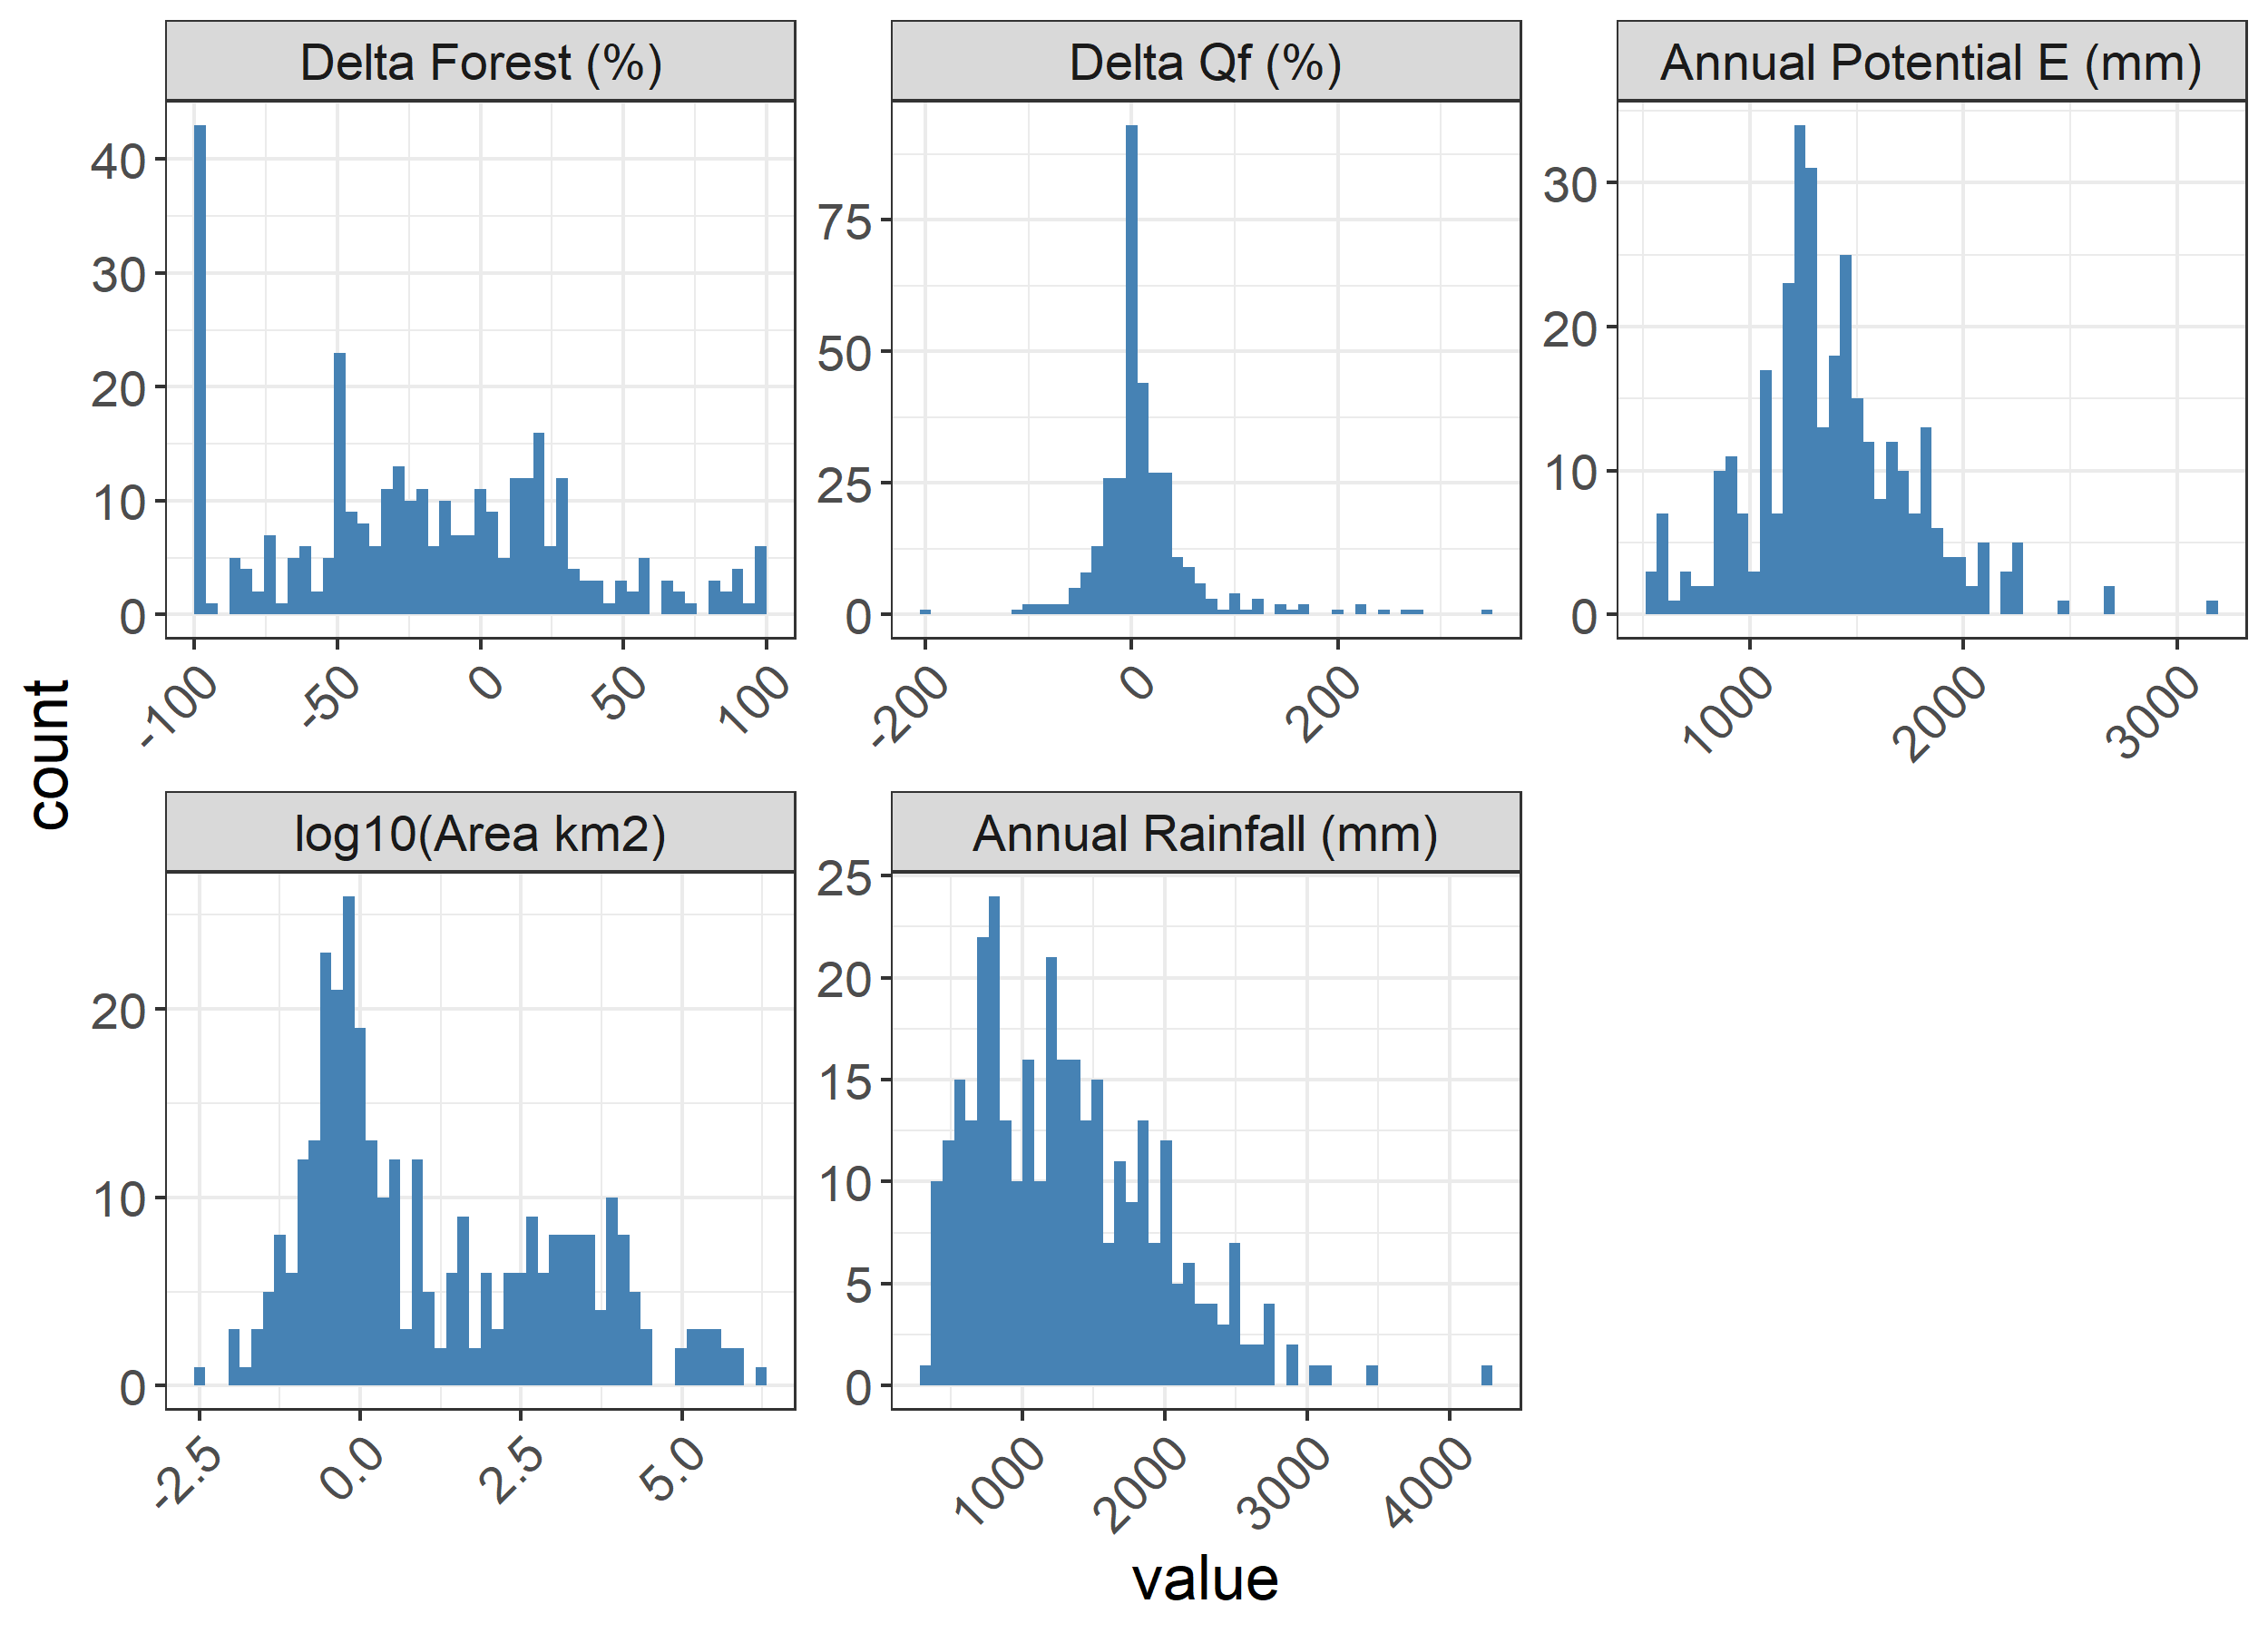
\includegraphics[width=0.9\linewidth]{./DataExploration} \caption{foo}\label{fig:datagraphs}
\end{figure}

\begin{figure}
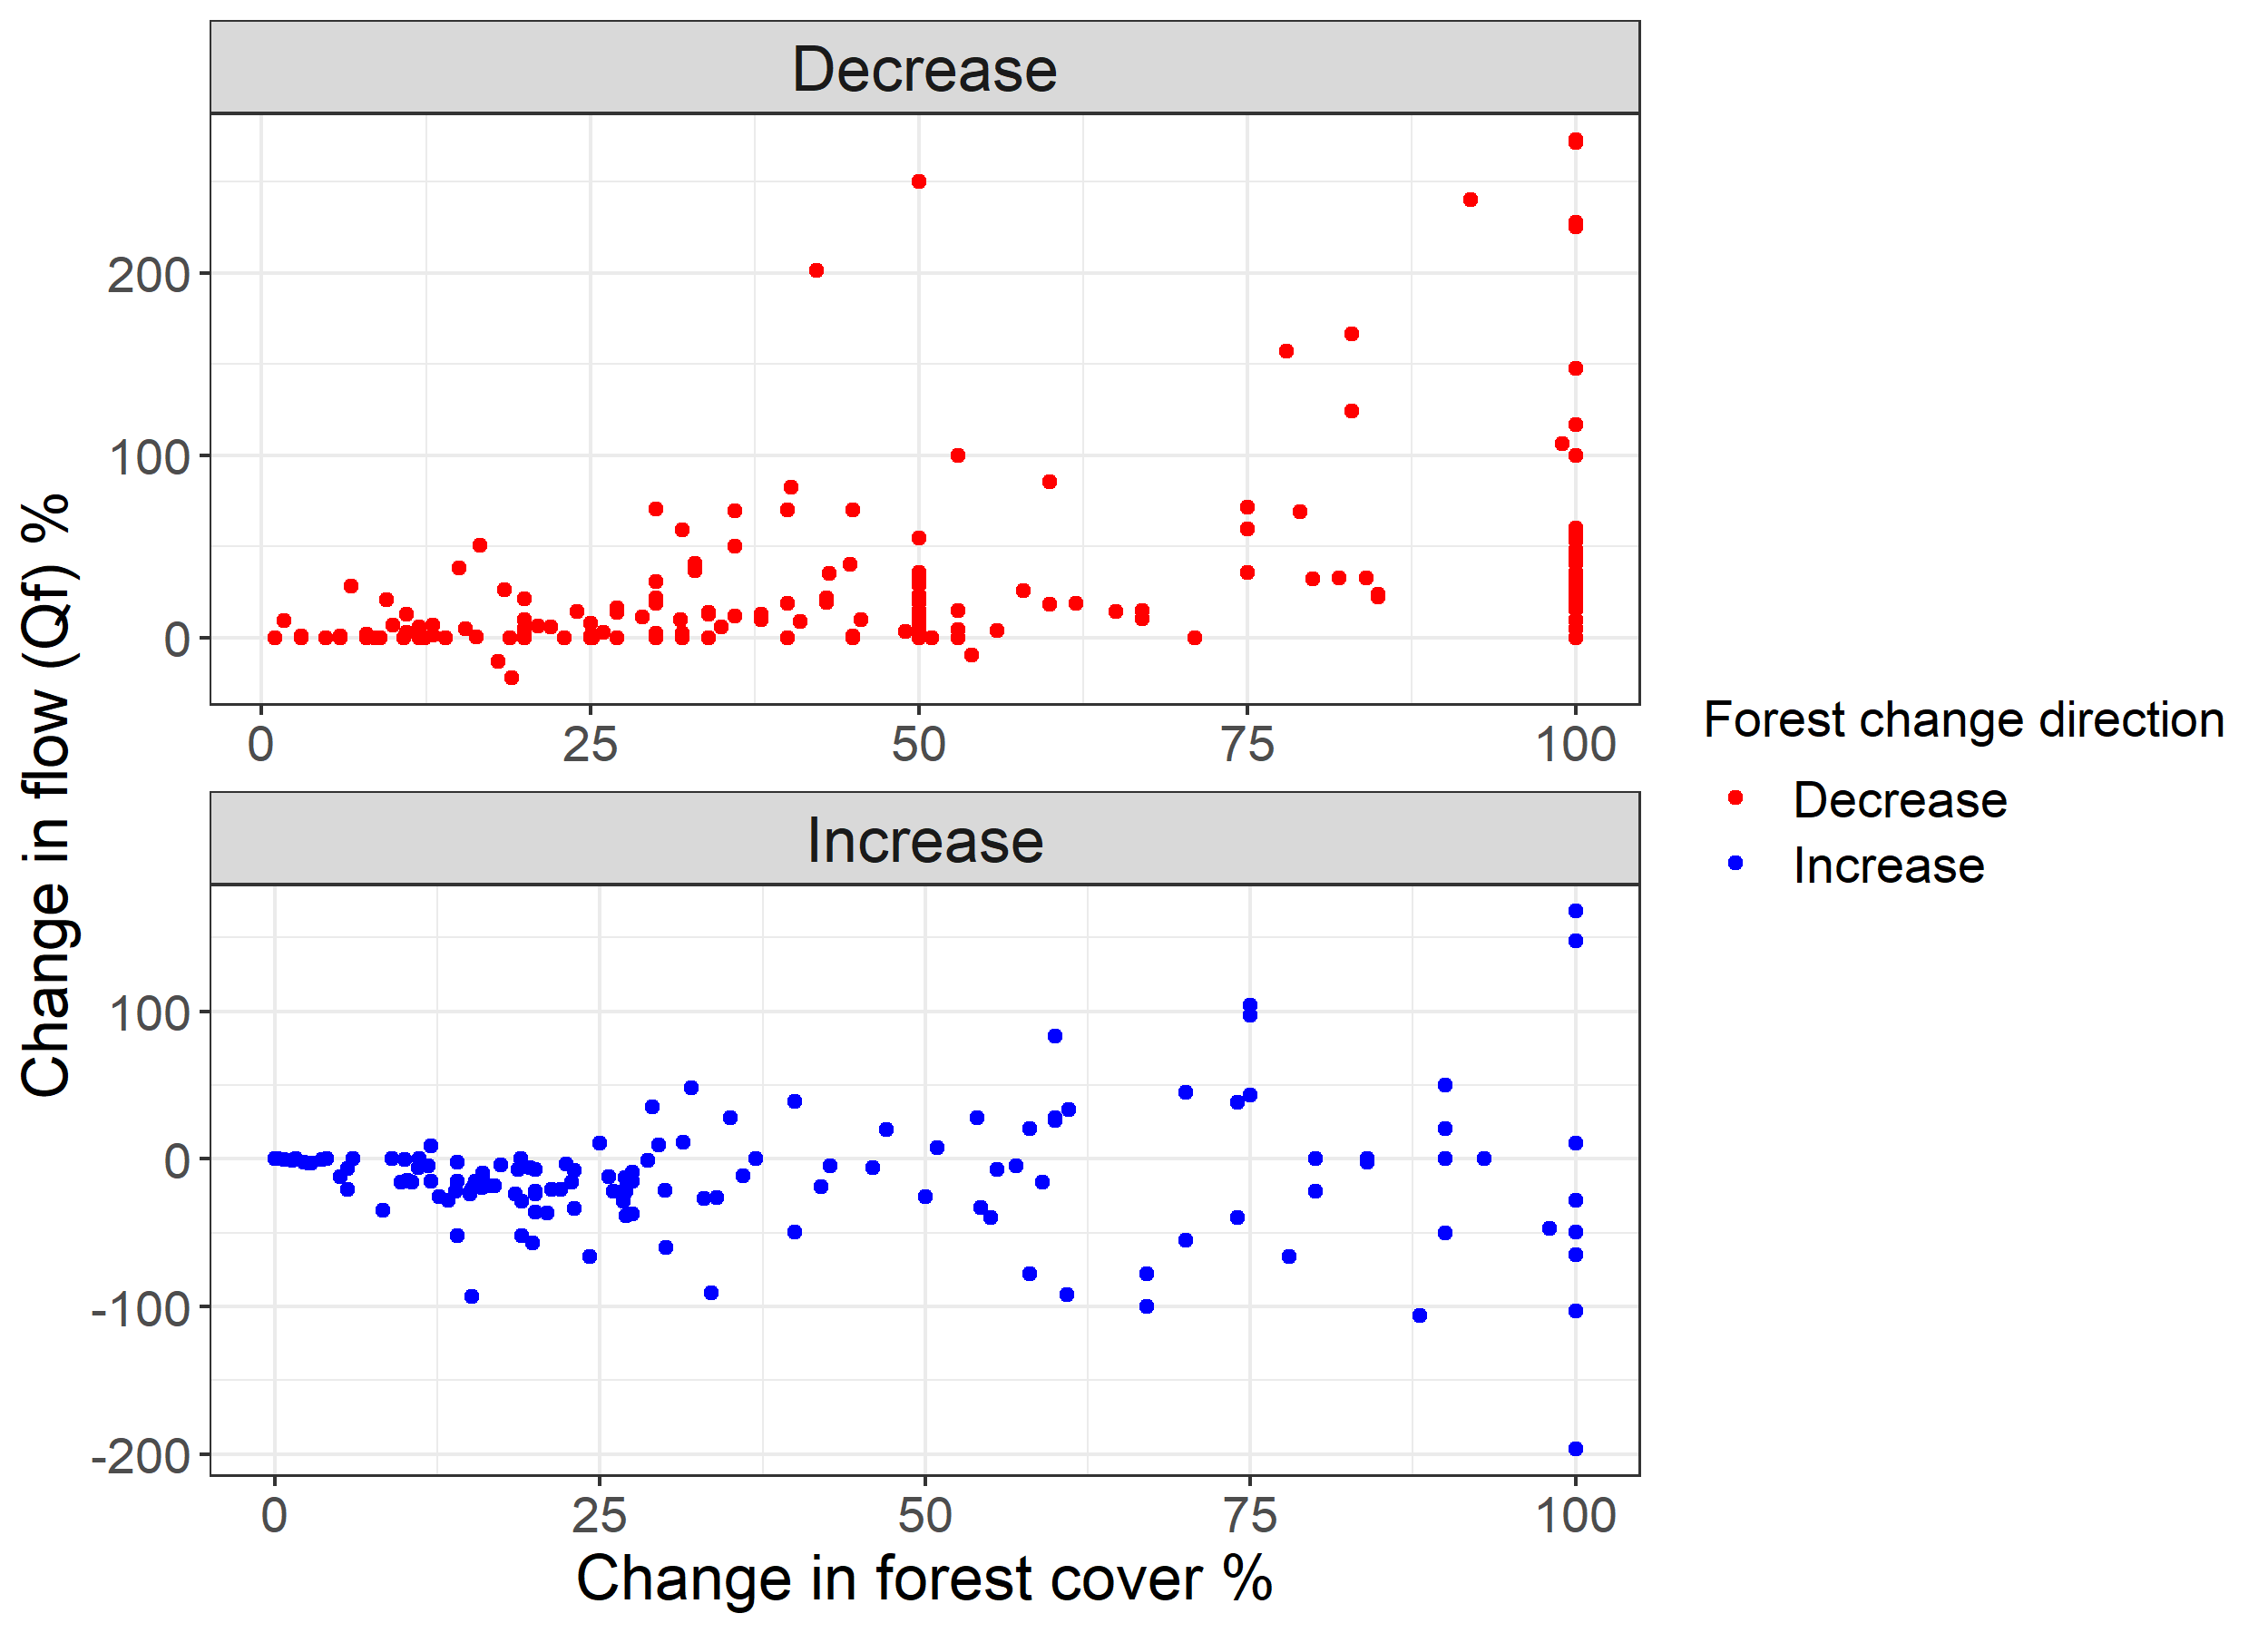
\includegraphics[width=0.9\linewidth]{Increase_decrease} \caption{Changes in flow as a function of increases and decreases in forest cover}\label{fig:increasedecrease}
\end{figure}

This shows that for the data related to forest decreases, there is almost always a positive flow change. In other words, flow almost always increased. However, for increases in forest cover, this is not the case, and flow can both increase and decrease. However in both cases the variability in the reported change in flow increases with the increase in forest cover change.

\hypertarget{the-general-relationship-between-change-in-forest-cover-and-streamflow}{%
\subsection{The general relationship between change in forest cover and streamflow}\label{the-general-relationship-between-change-in-forest-cover-and-streamflow}}

Following Zhang et al. (2017), the first step is to investigate the percent change in flow as a linear effect of the percent change forestry and modulated by the direction of the change, either an increase in forest cover, or decrease in forest cover:

\[\tag{3}
\begin{aligned}
\Delta \% Qf \sim ~ &\Delta \% forest~cover_{positive} + sign_{forest~cover} + \varepsilon
\end{aligned}\]

\begin{longtable}[]{@{}
  >{\centering\arraybackslash}p{(\columnwidth - 8\tabcolsep) * \real{0.36}}
  >{\centering\arraybackslash}p{(\columnwidth - 8\tabcolsep) * \real{0.15}}
  >{\centering\arraybackslash}p{(\columnwidth - 8\tabcolsep) * \real{0.18}}
  >{\centering\arraybackslash}p{(\columnwidth - 8\tabcolsep) * \real{0.14}}
  >{\centering\arraybackslash}p{(\columnwidth - 8\tabcolsep) * \real{0.15}}@{}}
\caption{\label{tab:tabmodel1} Summary results of the first regression model predicting change in streamflow from change in forest cover and accounting for the direction of the change}\tabularnewline
\toprule
\begin{minipage}[b]{\linewidth}\centering
~
\end{minipage} & \begin{minipage}[b]{\linewidth}\centering
Estimate
\end{minipage} & \begin{minipage}[b]{\linewidth}\centering
Std. Error
\end{minipage} & \begin{minipage}[b]{\linewidth}\centering
t value
\end{minipage} & \begin{minipage}[b]{\linewidth}\centering
Pr(\textgreater\textbar t\textbar)
\end{minipage} \\
\midrule
\endfirsthead
\toprule
\begin{minipage}[b]{\linewidth}\centering
~
\end{minipage} & \begin{minipage}[b]{\linewidth}\centering
Estimate
\end{minipage} & \begin{minipage}[b]{\linewidth}\centering
Std. Error
\end{minipage} & \begin{minipage}[b]{\linewidth}\centering
t value
\end{minipage} & \begin{minipage}[b]{\linewidth}\centering
Pr(\textgreater\textbar t\textbar)
\end{minipage} \\
\midrule
\endhead
\textbf{(Intercept)} & 8.65 & 5.56 & 1.56 & 0.12 \\
\textbf{DeltaF\_perc\_pos} & 0.45 & 0.09 & 5.26 & 0 \\
\textbf{Forest\_Signincrease} & -29.17 & 5.79 & -5.04 & 0 \\
\bottomrule
\end{longtable}

\begin{longtable}[]{@{}
  >{\centering\arraybackslash}p{(\columnwidth - 8\tabcolsep) * \real{0.36}}
  >{\centering\arraybackslash}p{(\columnwidth - 8\tabcolsep) * \real{0.15}}
  >{\centering\arraybackslash}p{(\columnwidth - 8\tabcolsep) * \real{0.18}}
  >{\centering\arraybackslash}p{(\columnwidth - 8\tabcolsep) * \real{0.14}}
  >{\centering\arraybackslash}p{(\columnwidth - 8\tabcolsep) * \real{0.15}}@{}}
\caption{\label{tab:tabmodel1b} Summary results of the first regression model predicting change in streamflow from change in forest cover and accounting for the direction of the change including the new data sets}\tabularnewline
\toprule
\begin{minipage}[b]{\linewidth}\centering
~
\end{minipage} & \begin{minipage}[b]{\linewidth}\centering
Estimate
\end{minipage} & \begin{minipage}[b]{\linewidth}\centering
Std. Error
\end{minipage} & \begin{minipage}[b]{\linewidth}\centering
t value
\end{minipage} & \begin{minipage}[b]{\linewidth}\centering
Pr(\textgreater\textbar t\textbar)
\end{minipage} \\
\midrule
\endfirsthead
\toprule
\begin{minipage}[b]{\linewidth}\centering
~
\end{minipage} & \begin{minipage}[b]{\linewidth}\centering
Estimate
\end{minipage} & \begin{minipage}[b]{\linewidth}\centering
Std. Error
\end{minipage} & \begin{minipage}[b]{\linewidth}\centering
t value
\end{minipage} & \begin{minipage}[b]{\linewidth}\centering
Pr(\textgreater\textbar t\textbar)
\end{minipage} \\
\midrule
\endhead
\textbf{(Intercept)} & 9.43 & 5.54 & 1.7 & 0.09 \\
\textbf{DeltaF\_perc\_pos} & 0.44 & 0.09 & 5.12 & 0 \\
\textbf{Forest\_Signincrease} & -36.54 & 5.59 & -6.53 & 0 \\
\bottomrule
\end{longtable}

The overall variance explained in this model is not high with an adjusted \emph{r\textsuperscript{2}} of 0.22, it generally supports the hypothesized relationship between the change in forest cover and the change in flow. The model suggests that for every 1\% change in forest cover, on the average, the flow changes 0.45\%. However the change in flow is different for forest cover decreases compared to forest cover increases. In fact, forest cover increases decrease flow by 29\% less than a similar decrease in forest cover causes flow to increase. So roughly speaking, a 1\% forest cover increase on the average decreases flow by \((1 - 0.29)*0.45\%\), while a the percentage forest cover decrease will increase flow by 0.45\%.

\begin{figure}
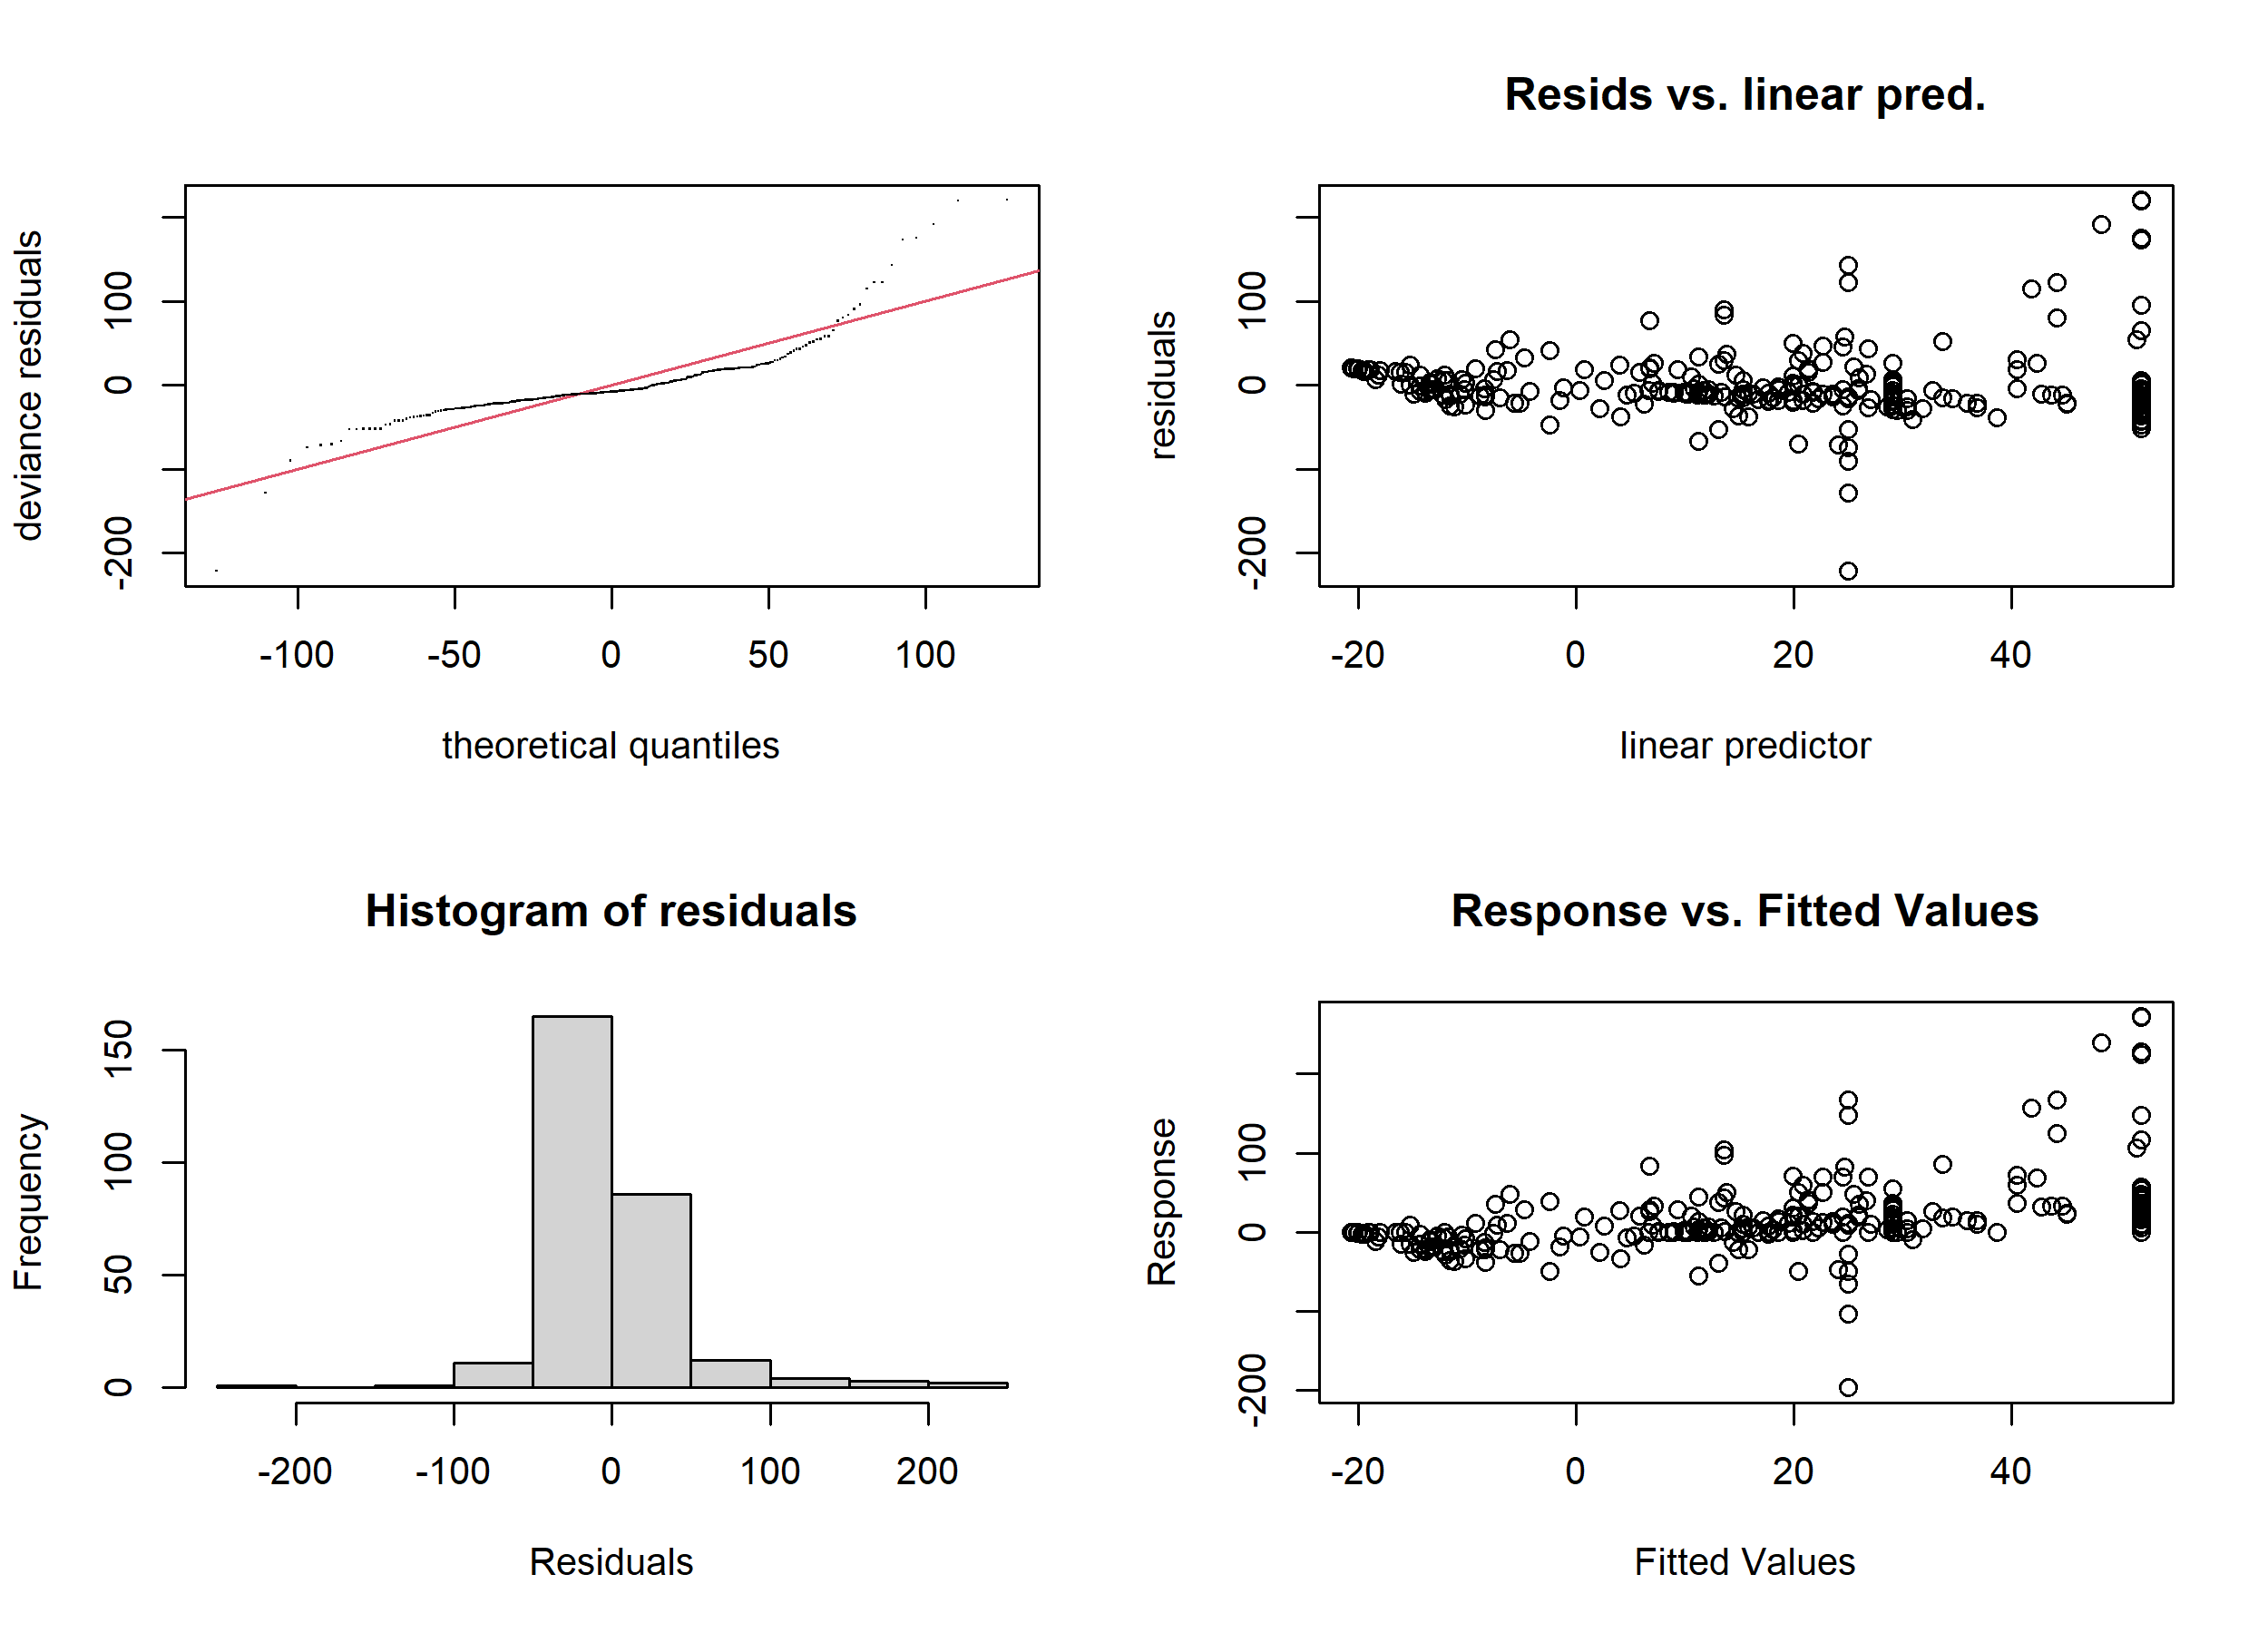
\includegraphics[width=0.9\linewidth]{residual_plot_model1} \caption{Residual plots for the first simple regression model indicating a slightly fat-tailed residual distribution}\label{fig:gamcheck}
\end{figure}

Of importance here is to highlight the residuals of this regression. These are approximately normal, although there is still significant skew on the upper and lower parts of the distribution (Figure \ref{fig:gamcheck}). In other words, the distribution of the residuals is somewhat fat-tailed. We will discuss this later.

Including the data from some of the newly identified studies indicates that this mainly strengthens the difference between the forest cover increases and decreases (Table \ref{tab:tabmodel1} and Table \ref{tab:tabmodel1b}), and the result indication a reduction in the mean decrease in flow as a result of forest cover change if the new data is included.

It is however it is clear from the lack of explaining power for the model, that there could be confounding factors, as alluded to in the methods. The obvious ones being watershed dryness and area (following Zhang et al. (2017)):

\[\tag{4}
\begin{aligned}
\Delta \% Qf \sim ~ &\Delta \% forest~cover_{positive} + sign_{forest~cover} + \\ & Pa_{mm} + log10(Area_{km^2}) + \varepsilon
\end{aligned}\]

Where \(Pa_mm\) is the annual average rainfall in mm, and a log base 10 transformation is applied to the area variable given that the distribution of Area is higly skewed (Figure 1)

\begin{longtable}[]{@{}
  >{\centering\arraybackslash}p{(\columnwidth - 8\tabcolsep) * \real{0.36}}
  >{\centering\arraybackslash}p{(\columnwidth - 8\tabcolsep) * \real{0.15}}
  >{\centering\arraybackslash}p{(\columnwidth - 8\tabcolsep) * \real{0.18}}
  >{\centering\arraybackslash}p{(\columnwidth - 8\tabcolsep) * \real{0.14}}
  >{\centering\arraybackslash}p{(\columnwidth - 8\tabcolsep) * \real{0.15}}@{}}
\caption{\label{tab:out-model2} Summary of the second model, taking into account the annual rainfall and the area of the watershed}\tabularnewline
\toprule
\begin{minipage}[b]{\linewidth}\centering
~
\end{minipage} & \begin{minipage}[b]{\linewidth}\centering
Estimate
\end{minipage} & \begin{minipage}[b]{\linewidth}\centering
Std. Error
\end{minipage} & \begin{minipage}[b]{\linewidth}\centering
t value
\end{minipage} & \begin{minipage}[b]{\linewidth}\centering
Pr(\textgreater\textbar t\textbar)
\end{minipage} \\
\midrule
\endfirsthead
\toprule
\begin{minipage}[b]{\linewidth}\centering
~
\end{minipage} & \begin{minipage}[b]{\linewidth}\centering
Estimate
\end{minipage} & \begin{minipage}[b]{\linewidth}\centering
Std. Error
\end{minipage} & \begin{minipage}[b]{\linewidth}\centering
t value
\end{minipage} & \begin{minipage}[b]{\linewidth}\centering
Pr(\textgreater\textbar t\textbar)
\end{minipage} \\
\midrule
\endhead
\textbf{(Intercept)} & 22.55 & 9.16 & 2.46 & 0.01 \\
\textbf{DeltaF\_perc\_pos} & 0.34 & 0.1 & 3.26 & 0 \\
\textbf{Forest\_Signincrease} & -35.52 & 5.67 & -6.27 & 0 \\
\textbf{log10(Area\_km2)} & -3.12 & 1.72 & -1.81 & 0.07 \\
\textbf{Pa\_mm} & 0 & 0 & -1 & 0.32 \\
\bottomrule
\end{longtable}

Including area and annual precipitation slightly improves the overall explaining power of the model (Table \ref{tab:out-model2}). Annual precipitation is in fact not significant. Relative to earlier reported studies (Filoso et al., 2017; Zhang et al., 2017), the log base 10 transformed watershed area indicates a p-value of only 0.07, suggesting a marginal impact on the change in stream flow. This supports our approach (in contrast to Zhang et al. (2017)) to consider watershed area as a continuous variable and making no separation between larger and smaller watersheds. The main effects in the model remain the change in forest cover and whether this is an increase or decrease.

\hypertarget{the-effect-of-location-on-the-globe}{%
\subsection{The effect of location on the globe}\label{the-effect-of-location-on-the-globe}}

\begin{figure}
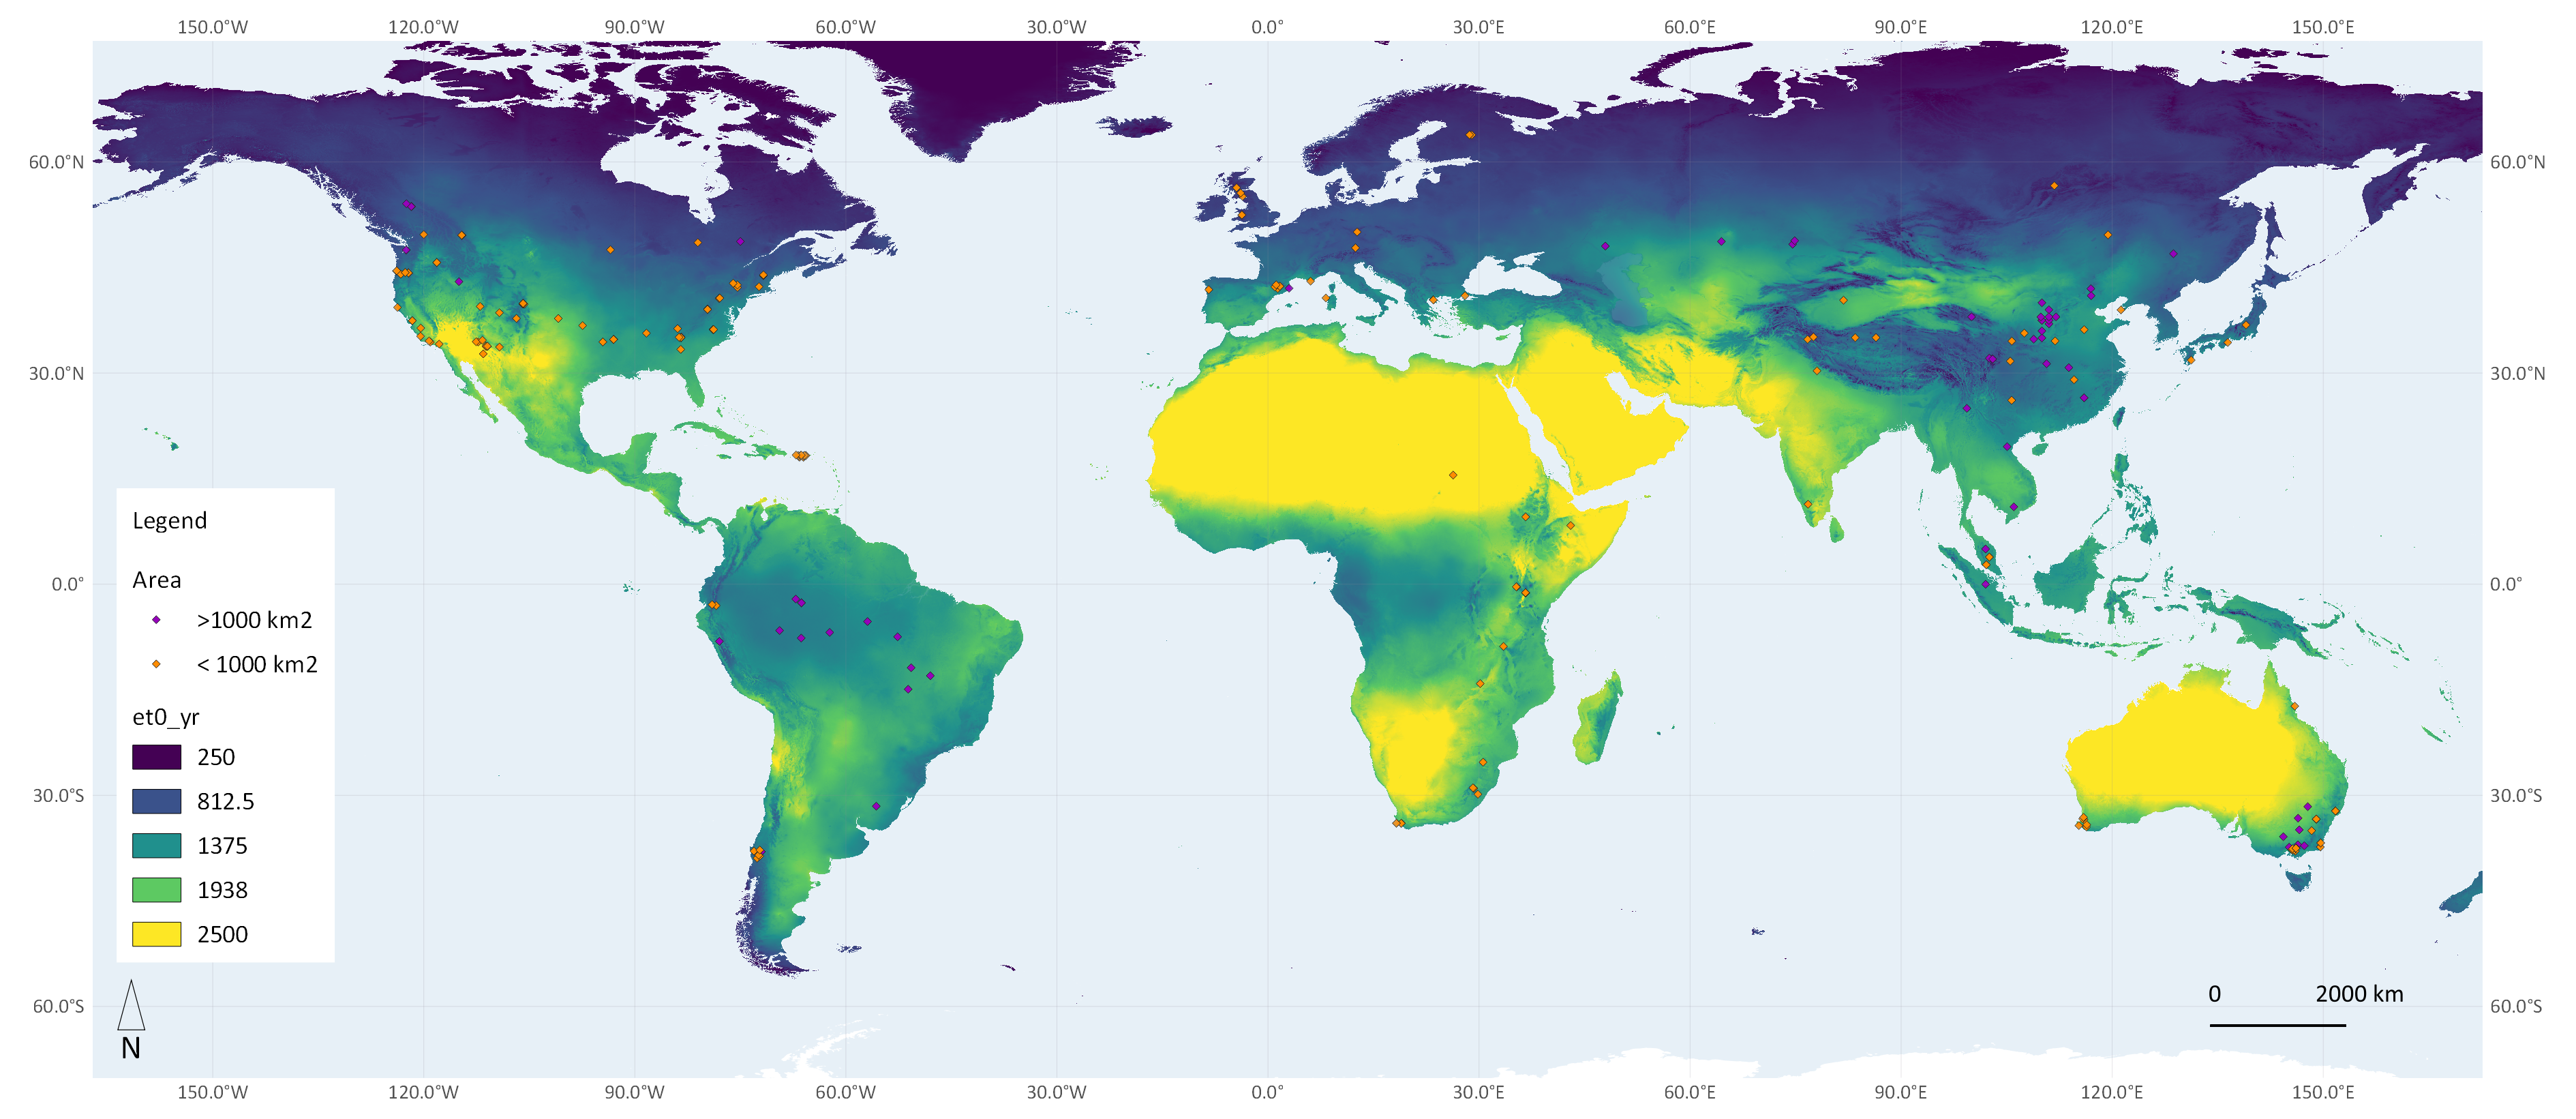
\includegraphics[width=0.9\linewidth]{../../data/FAOET0data2} \caption{Distribution of included watersheds across the globe based on reported or estimated latitude and longitude}\label{fig:globalmap}
\end{figure}

As indicated, a further hypothesis relates to whether there is a strong spatial global gradient as captured by latitude and longitude. As the global map (Figure \ref{fig:globalmap}) shows, the distribution of case study watersheds covers multiple continents and shows some distinct clustering in parts of the world. Of interest is whether the spatial clustering also indicates a difference in response to forest cover change:

\[\tag{5}
\begin{aligned}
\Delta \% Qf \sim ~ &\Delta \% forest~cover_{positive} + sign_{forest~cover} + \\ & Pa_{mm} + log10(Area_{km^2}) + Latitude + Longitude + \varepsilon
\end{aligned}\]

\begin{longtable}[]{@{}
  >{\centering\arraybackslash}p{(\columnwidth - 8\tabcolsep) * \real{0.36}}
  >{\centering\arraybackslash}p{(\columnwidth - 8\tabcolsep) * \real{0.15}}
  >{\centering\arraybackslash}p{(\columnwidth - 8\tabcolsep) * \real{0.18}}
  >{\centering\arraybackslash}p{(\columnwidth - 8\tabcolsep) * \real{0.14}}
  >{\centering\arraybackslash}p{(\columnwidth - 8\tabcolsep) * \real{0.15}}@{}}
\caption{\label{tab:out-model3} Results of the model including Latitude and Longitude including new data}\tabularnewline
\toprule
\begin{minipage}[b]{\linewidth}\centering
~
\end{minipage} & \begin{minipage}[b]{\linewidth}\centering
Estimate
\end{minipage} & \begin{minipage}[b]{\linewidth}\centering
Std. Error
\end{minipage} & \begin{minipage}[b]{\linewidth}\centering
t value
\end{minipage} & \begin{minipage}[b]{\linewidth}\centering
Pr(\textgreater\textbar t\textbar)
\end{minipage} \\
\midrule
\endfirsthead
\toprule
\begin{minipage}[b]{\linewidth}\centering
~
\end{minipage} & \begin{minipage}[b]{\linewidth}\centering
Estimate
\end{minipage} & \begin{minipage}[b]{\linewidth}\centering
Std. Error
\end{minipage} & \begin{minipage}[b]{\linewidth}\centering
t value
\end{minipage} & \begin{minipage}[b]{\linewidth}\centering
Pr(\textgreater\textbar t\textbar)
\end{minipage} \\
\midrule
\endhead
\textbf{(Intercept)} & 23.29 & 9.96 & 2.34 & 0.02 \\
\textbf{DeltaF\_perc\_pos} & 0.35 & 0.1 & 3.32 & 0 \\
\textbf{Forest\_Signincrease} & -37.21 & 6 & -6.2 & 0 \\
\textbf{log10(Area\_km2)} & -3.28 & 1.73 & -1.89 & 0.06 \\
\textbf{Pa\_mm} & 0 & 0 & -0.83 & 0.41 \\
\textbf{Latitude} & -0.05 & 0.09 & -0.55 & 0.58 \\
\textbf{Longitude} & 0.01 & 0.03 & 0.23 & 0.82 \\
\bottomrule
\end{longtable}

There appears to be no significant gradient in either latitude or longitude (Table \ref{tab:out-model3}), suggesting that the distribution of the watersheds across the globe has little influence on the overall result. The total explaining power of the model is still low with an adjusted \emph{r\textsuperscript{2}} of 0.22 suggesting further factors influencing the change in streamflow that are currently not included in the model.

Note that in this case the significance of the Area variable increases, and generally indicates that larger watersheds would be expected to have a lower change in streamflow, as also indicated in Zhang et al. (2017).

\hypertarget{impact-of-the-dryness-index}{%
\subsection{Impact of the dryness index}\label{impact-of-the-dryness-index}}

Climate, and in particular evapotranspiration can have a significant effect on the streamflow change as represented by the dryness index, which is also highlghted by both Zhang et al. (2017) and Jackson et al. (2005). Increased evapotranspiration could lead to drier watersheds, unless balanced by rainfall (such as possibly in the tropics). This model introduces the dryness index as a linear variable and drops the annual average precipitation as a variable, as dryness is calculated from the precipitation. It also drops the Latitude and Longitude as these are indicated not to be significant.

\begin{longtable}[]{@{}
  >{\centering\arraybackslash}p{(\columnwidth - 8\tabcolsep) * \real{0.36}}
  >{\centering\arraybackslash}p{(\columnwidth - 8\tabcolsep) * \real{0.15}}
  >{\centering\arraybackslash}p{(\columnwidth - 8\tabcolsep) * \real{0.18}}
  >{\centering\arraybackslash}p{(\columnwidth - 8\tabcolsep) * \real{0.14}}
  >{\centering\arraybackslash}p{(\columnwidth - 8\tabcolsep) * \real{0.15}}@{}}
\caption{\label{tab:out-model4} Results of the model replacing the annual precipitation with the dryness index}\tabularnewline
\toprule
\begin{minipage}[b]{\linewidth}\centering
~
\end{minipage} & \begin{minipage}[b]{\linewidth}\centering
Estimate
\end{minipage} & \begin{minipage}[b]{\linewidth}\centering
Std. Error
\end{minipage} & \begin{minipage}[b]{\linewidth}\centering
t value
\end{minipage} & \begin{minipage}[b]{\linewidth}\centering
Pr(\textgreater\textbar t\textbar)
\end{minipage} \\
\midrule
\endfirsthead
\toprule
\begin{minipage}[b]{\linewidth}\centering
~
\end{minipage} & \begin{minipage}[b]{\linewidth}\centering
Estimate
\end{minipage} & \begin{minipage}[b]{\linewidth}\centering
Std. Error
\end{minipage} & \begin{minipage}[b]{\linewidth}\centering
t value
\end{minipage} & \begin{minipage}[b]{\linewidth}\centering
Pr(\textgreater\textbar t\textbar)
\end{minipage} \\
\midrule
\endhead
\textbf{(Intercept)} & 10.46 & 7.66 & 1.36 & 0.17 \\
\textbf{DeltaF\_perc\_pos} & 0.31 & 0.11 & 2.93 & 0 \\
\textbf{Forest\_Signincrease} & -35.67 & 5.73 & -6.23 & 0 \\
\textbf{log10(Area\_km2)} & -3.5 & 1.76 & -1.99 & 0.05 \\
\textbf{Dryness} & 6.54 & 3.08 & 2.12 & 0.03 \\
\bottomrule
\end{longtable}

The results from this model (Table \ref{tab:out-model4}) confirm that dryness is a significant confounding factor related to the change in streamflow as a function of the change in forest cover change. In fact if the dryness index doubles (remembering that Dryness = 1 when E0 = Pa, so in this case E0 = 2*Pa, which is very dry), the change in runoff is \textasciitilde14\% greater. However, more interesting, Latitude remains a significant predictor with each degree in latitude causing an -0.31\% change in runoff. This indicates that Dryness (i.e.~an increase in radiation) alone does not explain the trend in the Latitude and some other unknown confounding factor is captured by Latitude.

\begin{longtable}[]{@{}
  >{\centering\arraybackslash}p{(\columnwidth - 4\tabcolsep) * \real{0.15}}
  >{\centering\arraybackslash}p{(\columnwidth - 4\tabcolsep) * \real{0.17}}
  >{\centering\arraybackslash}p{(\columnwidth - 4\tabcolsep) * \real{0.46}}@{}}
\caption{\label{tab:drytable} Watersheds for which the dryness index \textgreater{} 4}\tabularnewline
\toprule
\begin{minipage}[b]{\linewidth}\centering
Latitude
\end{minipage} & \begin{minipage}[b]{\linewidth}\centering
Longitude
\end{minipage} & \begin{minipage}[b]{\linewidth}\centering
Watershed name
\end{minipage} \\
\midrule
\endfirsthead
\toprule
\begin{minipage}[b]{\linewidth}\centering
Latitude
\end{minipage} & \begin{minipage}[b]{\linewidth}\centering
Longitude
\end{minipage} & \begin{minipage}[b]{\linewidth}\centering
Watershed name
\end{minipage} \\
\midrule
\endhead
34.67 & -111.7 & Beaver Creek, AZ \#3-2 \\
36.4 & -120.4 & Cantua \\
34.43 & -112.3 & White Spar, Ariz., U.S.A, B \\
32.74 & -111.5 & Natural DRDages, Ariz., U.S.A,
A \\
\bottomrule
\end{longtable}

However, the result also indicates possible issues with the data, some of the Dryness values are very large (\textgreater{} 4) and these values have high leverage in the data. These watersheds are listed in Table \ref{tab:drytable}.

\hypertarget{are-some-of-the-variables-possibly-non-linear}{%
\subsubsection{Are some of the variables possibly non-linear?}\label{are-some-of-the-variables-possibly-non-linear}}

The work by Filoso et al. (2017) and earlier by Jackson et al. (2005) has indicated that the length of the study might influence the response. This links to the idea from Kuczera (1987) that the effect of logging or deforestation or reforestation reduces with the length of time post intervention (see also Jackson et al. (2005)). In addition to adding the length as a variable, all continuous variables (Dryness, Area, length and Latitude) were considered non-linear in this model and as indicated a shrinkage smoothing spline (Wood, 2006) was applied to these variables.

\begin{longtable}[]{@{}
  >{\centering\arraybackslash}p{(\columnwidth - 8\tabcolsep) * \real{0.36}}
  >{\centering\arraybackslash}p{(\columnwidth - 8\tabcolsep) * \real{0.15}}
  >{\centering\arraybackslash}p{(\columnwidth - 8\tabcolsep) * \real{0.18}}
  >{\centering\arraybackslash}p{(\columnwidth - 8\tabcolsep) * \real{0.14}}
  >{\centering\arraybackslash}p{(\columnwidth - 8\tabcolsep) * \real{0.15}}@{}}
\caption{Statistical summary for the linear terms in the model with non-linear terms}\tabularnewline
\toprule
\begin{minipage}[b]{\linewidth}\centering
~
\end{minipage} & \begin{minipage}[b]{\linewidth}\centering
Estimate
\end{minipage} & \begin{minipage}[b]{\linewidth}\centering
Std. Error
\end{minipage} & \begin{minipage}[b]{\linewidth}\centering
t value
\end{minipage} & \begin{minipage}[b]{\linewidth}\centering
Pr(\textgreater\textbar t\textbar)
\end{minipage} \\
\midrule
\endfirsthead
\toprule
\begin{minipage}[b]{\linewidth}\centering
~
\end{minipage} & \begin{minipage}[b]{\linewidth}\centering
Estimate
\end{minipage} & \begin{minipage}[b]{\linewidth}\centering
Std. Error
\end{minipage} & \begin{minipage}[b]{\linewidth}\centering
t value
\end{minipage} & \begin{minipage}[b]{\linewidth}\centering
Pr(\textgreater\textbar t\textbar)
\end{minipage} \\
\midrule
\endhead
\textbf{(Intercept)} & 17.09 & 6.08 & 2.81 & 0.01 \\
\textbf{DeltaF\_perc\_pos} & 0.26 & 0.11 & 2.44 & 0.02 \\
\textbf{Forest\_Signincrease} & -34.6 & 6.11 & -5.67 & 0 \\
\bottomrule
\end{longtable}

\begin{longtable}[]{@{}
  >{\centering\arraybackslash}p{(\columnwidth - 8\tabcolsep) * \real{0.35}}
  >{\centering\arraybackslash}p{(\columnwidth - 8\tabcolsep) * \real{0.10}}
  >{\centering\arraybackslash}p{(\columnwidth - 8\tabcolsep) * \real{0.12}}
  >{\centering\arraybackslash}p{(\columnwidth - 8\tabcolsep) * \real{0.10}}
  >{\centering\arraybackslash}p{(\columnwidth - 8\tabcolsep) * \real{0.14}}@{}}
\caption{Statistical summary for the smooth terms in the model with non-linear terms}\tabularnewline
\toprule
\begin{minipage}[b]{\linewidth}\centering
~
\end{minipage} & \begin{minipage}[b]{\linewidth}\centering
edf
\end{minipage} & \begin{minipage}[b]{\linewidth}\centering
Ref.df
\end{minipage} & \begin{minipage}[b]{\linewidth}\centering
F
\end{minipage} & \begin{minipage}[b]{\linewidth}\centering
p-value
\end{minipage} \\
\midrule
\endfirsthead
\toprule
\begin{minipage}[b]{\linewidth}\centering
~
\end{minipage} & \begin{minipage}[b]{\linewidth}\centering
edf
\end{minipage} & \begin{minipage}[b]{\linewidth}\centering
Ref.df
\end{minipage} & \begin{minipage}[b]{\linewidth}\centering
F
\end{minipage} & \begin{minipage}[b]{\linewidth}\centering
p-value
\end{minipage} \\
\midrule
\endhead
\textbf{s(log10(Area\_km2))} & 1.74 & 9 & 0.78 & 0.01 \\
\textbf{s(Dryness)} & 0.87 & 9 & 0.57 & 0.02 \\
\textbf{s(length)} & 8.83 & 9 & 3.1 & 0 \\
\bottomrule
\end{longtable}

Including non-linearity increases the overall explaining power of the model to an adjusted \emph{r\textsuperscript{2}} of 0.29 and deviance explained of 0.32, but creates few changes in the significance of the variables (Table \ref{tab:mfive-smooth}). However, it also increases the chance of over fitting, as the smoothing splines allow significant flexibility, which will be investigated later.

A final full model which includes the remaining categorical variables (Precipitation data type, Assessment technique, Forest type and Hydrological regime) is tested.

\begin{longtable}[]{@{}
  >{\centering\arraybackslash}p{(\columnwidth - 8\tabcolsep) * \real{0.42}}
  >{\centering\arraybackslash}p{(\columnwidth - 8\tabcolsep) * \real{0.14}}
  >{\centering\arraybackslash}p{(\columnwidth - 8\tabcolsep) * \real{0.17}}
  >{\centering\arraybackslash}p{(\columnwidth - 8\tabcolsep) * \real{0.13}}
  >{\centering\arraybackslash}p{(\columnwidth - 8\tabcolsep) * \real{0.14}}@{}}
\caption{Statistical summary for the linear terms the full model}\tabularnewline
\toprule
\begin{minipage}[b]{\linewidth}\centering
~
\end{minipage} & \begin{minipage}[b]{\linewidth}\centering
Estimate
\end{minipage} & \begin{minipage}[b]{\linewidth}\centering
Std. Error
\end{minipage} & \begin{minipage}[b]{\linewidth}\centering
t value
\end{minipage} & \begin{minipage}[b]{\linewidth}\centering
Pr(\textgreater\textbar t\textbar)
\end{minipage} \\
\midrule
\endfirsthead
\toprule
\begin{minipage}[b]{\linewidth}\centering
~
\end{minipage} & \begin{minipage}[b]{\linewidth}\centering
Estimate
\end{minipage} & \begin{minipage}[b]{\linewidth}\centering
Std. Error
\end{minipage} & \begin{minipage}[b]{\linewidth}\centering
t value
\end{minipage} & \begin{minipage}[b]{\linewidth}\centering
Pr(\textgreater\textbar t\textbar)
\end{minipage} \\
\midrule
\endhead
\textbf{(Intercept)} & -27.3 & 19.84 & -1.38 & 0.17 \\
\textbf{DeltaF\_perc\_pos} & 0.31 & 0.1 & 3.01 & 0 \\
\textbf{Forest\_Signincrease} & -21.54 & 7.29 & -2.96 & 0 \\
\textbf{Precip\_data\_typeOB} & -8.13 & 15.17 & -0.54 & 0.59 \\
\textbf{Precip\_data\_typeSG} & 17.33 & 17.29 & 1 & 0.32 \\
\textbf{Assessment\_techniqueEA, HM} & 13.93 & 46.74 & 0.3 & 0.77 \\
\textbf{Assessment\_techniqueHM} & 32.96 & 13.92 & 2.37 & 0.02 \\
\textbf{Assessment\_techniquePWE} & 53.24 & 12.81 & 4.16 & 0 \\
\textbf{Assessment\_techniquePWE,
HM} & 33.54 & 47.07 & 0.71 & 0.48 \\
\textbf{Assessment\_techniqueQPW} & 39.8 & 22.06 & 1.8 & 0.07 \\
\textbf{Assessment\_techniqueQPW,
EA} & 45.97 & 26.25 & 1.75 & 0.08 \\
\textbf{Assessment\_techniqueSH} & 44.89 & 13.49 & 3.33 & 0 \\
\textbf{Forest\_typeCF} & -2.2 & 8.52 & -0.26 & 0.8 \\
\textbf{Forest\_typeMF} & -6.56 & 8.96 & -0.73 & 0.46 \\
\textbf{Hydrological\_regimeSD} & 4.59 & 10.25 & 0.45 & 0.65 \\
\bottomrule
\end{longtable}

\begin{Shaded}
\begin{Highlighting}[]
\FunctionTok{pander}\NormalTok{(}\FunctionTok{round}\NormalTok{(}\FunctionTok{summary}\NormalTok{(model6\_all)}\SpecialCharTok{$}\NormalTok{s.table,}\DecValTok{2}\NormalTok{), }\AttributeTok{caption =} \StringTok{"Statistical summary for the smooth terms for the full model"}\NormalTok{)}
\end{Highlighting}
\end{Shaded}

\begin{longtable}[]{@{}
  >{\centering\arraybackslash}p{(\columnwidth - 8\tabcolsep) * \real{0.35}}
  >{\centering\arraybackslash}p{(\columnwidth - 8\tabcolsep) * \real{0.10}}
  >{\centering\arraybackslash}p{(\columnwidth - 8\tabcolsep) * \real{0.12}}
  >{\centering\arraybackslash}p{(\columnwidth - 8\tabcolsep) * \real{0.10}}
  >{\centering\arraybackslash}p{(\columnwidth - 8\tabcolsep) * \real{0.14}}@{}}
\caption{Statistical summary for the smooth terms for the full model}\tabularnewline
\toprule
\begin{minipage}[b]{\linewidth}\centering
~
\end{minipage} & \begin{minipage}[b]{\linewidth}\centering
edf
\end{minipage} & \begin{minipage}[b]{\linewidth}\centering
Ref.df
\end{minipage} & \begin{minipage}[b]{\linewidth}\centering
F
\end{minipage} & \begin{minipage}[b]{\linewidth}\centering
p-value
\end{minipage} \\
\midrule
\endfirsthead
\toprule
\begin{minipage}[b]{\linewidth}\centering
~
\end{minipage} & \begin{minipage}[b]{\linewidth}\centering
edf
\end{minipage} & \begin{minipage}[b]{\linewidth}\centering
Ref.df
\end{minipage} & \begin{minipage}[b]{\linewidth}\centering
F
\end{minipage} & \begin{minipage}[b]{\linewidth}\centering
p-value
\end{minipage} \\
\midrule
\endhead
\textbf{s(log10(Area\_km2))} & 0.31 & 9 & 0.07 & 0.16 \\
\textbf{s(Dryness)} & 3.45 & 9 & 1.39 & 0.01 \\
\textbf{s(length)} & 8.73 & 9 & 3.04 & 0 \\
\bottomrule
\end{longtable}

\begin{Shaded}
\begin{Highlighting}[]
\CommentTok{\#plot(model6\_all)}
\end{Highlighting}
\end{Shaded}

This model explains more of the variance, but the improvement is marginal compared to the previous model with a deviance explained of 0.38. This indicates that the categorical variables explain a limited amount of the variance. However, interesting to note from Table \ref{tab:msix-linear} that several of the assessment methods are significant. In particular Paired Watersheds experiments (PWE), Hydrological modelling (HM) and Statistical techniques (SH) are strongly significant (\(p < 0.05\)).

\begin{figure}
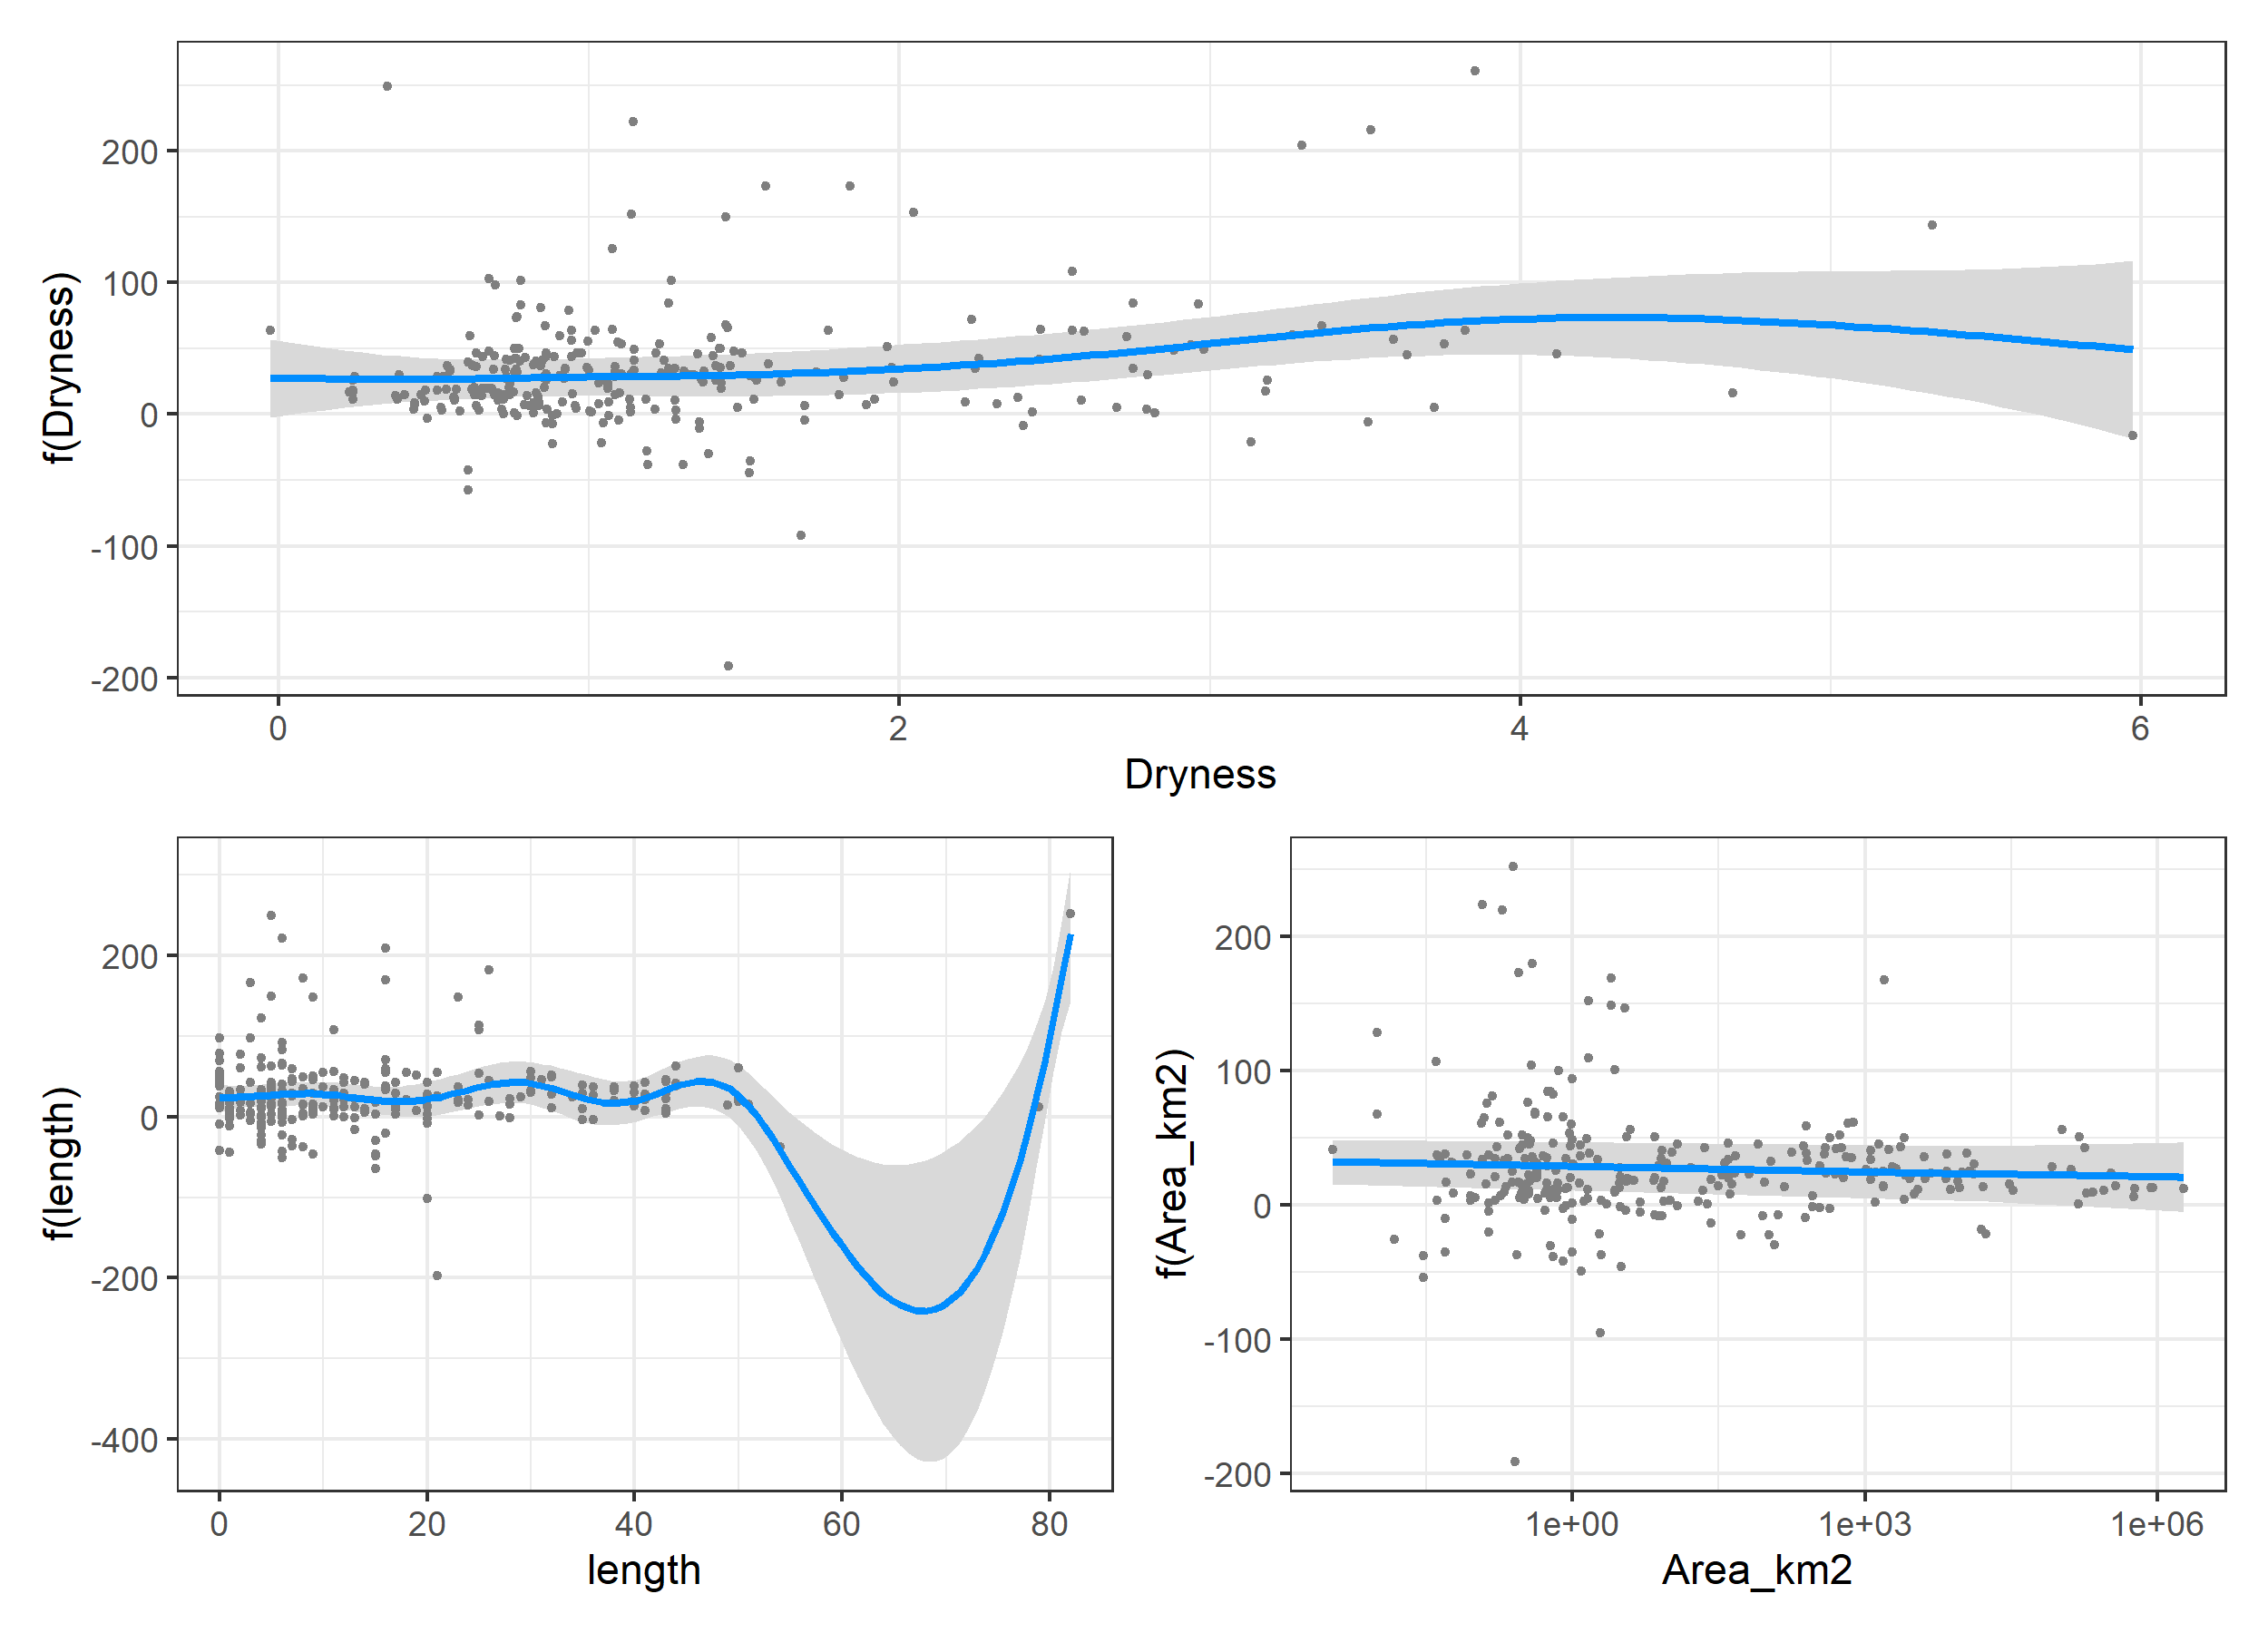
\includegraphics[width=0.9\linewidth]{model6_smooths} \caption{Visualisation of the smooth variables in the model}\label{fig:smoothsmodel6}
\end{figure}

Figure \ref{fig:smoothsmodel6} highlights that the relationship between log10(Area) and the change in flow is essentially linear and does not need to be smoothed (this is the value of using penalized smooths following Wood (2006)). It is still a negative slope, indicating that in larger watersheds the impact of changes in forest cover on streamflow is less than for smaller watersheds. In addition, both the length and Dryness variables show non-linearity, but this does not show a clear trend.

Quitting from lines 645-646 (Forest\_and\_Water.Rmd)
Error in summary(model7\_nolongLength) :
object `model7\_nolongLength' not found
Calls: \ldots{} withCallingHandlers -\textgreater{} withVisible -\textgreater{} eval -\textgreater{} eval -\textgreater{} pander -\textgreater{} summary
In addition: Warning messages:
1: In eval(expr, envir, enclos) : NAs introduced by coercion
2: In eval(expr, envir, enclos) : NAs introduced by coercion

The flexible nature of the splines means that the length variable captures some substantial variation in the data, but it is unclear what exactly is captured. The shape of the conditional response (Figure \ref{fig:smoothsmodel6}) also does not reflect the type of response highlighted in Filoso et al. (2017) and Jackson et al. (2005). One reason could be the few data points with very long data series, but highly variable responses (Figure \ref{fig:smoothsmodel6}). Reducing the flexibility of the splines, removing any studies longer than 60 years (Table \ref{tab:restrictlength}), or fitting a linear term results in ``length'' not being significant, suggesting that this variable is not helpful in explaining the variation in the data.

\begin{Shaded}
\begin{Highlighting}[]
\NormalTok{Zhang\_all2 }\SpecialCharTok{\%\textgreater{}\%}
  \FunctionTok{ggplot}\NormalTok{(}\FunctionTok{aes}\NormalTok{(length)) }\SpecialCharTok{+} \FunctionTok{geom\_histogram}\NormalTok{(}\AttributeTok{fill=}\StringTok{"blue"}\NormalTok{, }\AttributeTok{bins =}\DecValTok{50}\NormalTok{) }
\end{Highlighting}
\end{Shaded}

\hypertarget{discussion}{%
\section{Discussion}\label{discussion}}

Essentially, the analysis shows at the moment that in contrast to Zhang et al. (2017) there is no evidence that the size of a watershed influences the change in the streamflow as a result of changes in forestry. If anything the scatter in the data (in the change in flow) is greater for the smaller watersheds then for the larger watersheds. In other words, the response to changes in forest cover is more consistent for larger watersheds than it is for smaller watersheds.

As shown earlier, most of the smaller watersheds are ``real observed data'' using paired watershed studies, while for larger watersheds, the analysis are mostly based on modelling approximations using either elasticity analysis (EA), Hydrological modelling (HM) or a combined use of statistical methods (SH) or quasi paired watershed analysis (QPW), thus all providing an approximation of the effect of forestry on streamflow rather than a direct comparison of watersheds. This is a confounding factor that is not easily addressed in the regression modelling attempted here. Furthermore, the catchments analysed using EA, are concentrated in the drier end of the Dryness index scale compared to the other methods, with only the paired watershed experiment (PWE) assessment technique covering the full range of dryness indices.

\hypertarget{remove-the-assessment-techniques-with-very-small-numbers}{%
\subsubsection{remove the assessment techniques with very small numbers}\label{remove-the-assessment-techniques-with-very-small-numbers}}

One concern is that there are a few Assessment techniques in the original dataset with a very low number of observations and this might skew the results of the analysis. This includes the category of Quasi paired watersheds and combinations of elasticity analysis and hydrological modelling (EA,HM) and paired watersheds and hydrological modelling (PWE,HM).

\begin{longtable}[]{@{}
  >{\centering\arraybackslash}p{(\columnwidth - 2\tabcolsep) * \real{0.32}}
  >{\centering\arraybackslash}p{(\columnwidth - 2\tabcolsep) * \real{0.08}}@{}}
\toprule
\begin{minipage}[b]{\linewidth}\centering
Assessment\_technique
\end{minipage} & \begin{minipage}[b]{\linewidth}\centering
n
\end{minipage} \\
\midrule
\endhead
PWE & 185 \\
HM & 53 \\
EA & 32 \\
SH & 26 \\
QPW & 7 \\
QPW, EA & 4 \\
EA, HM & 1 \\
PWE, HM & 1 \\
\bottomrule
\end{longtable}

\begin{verbatim}
## pdf 
##   2
\end{verbatim}

\begin{figure}
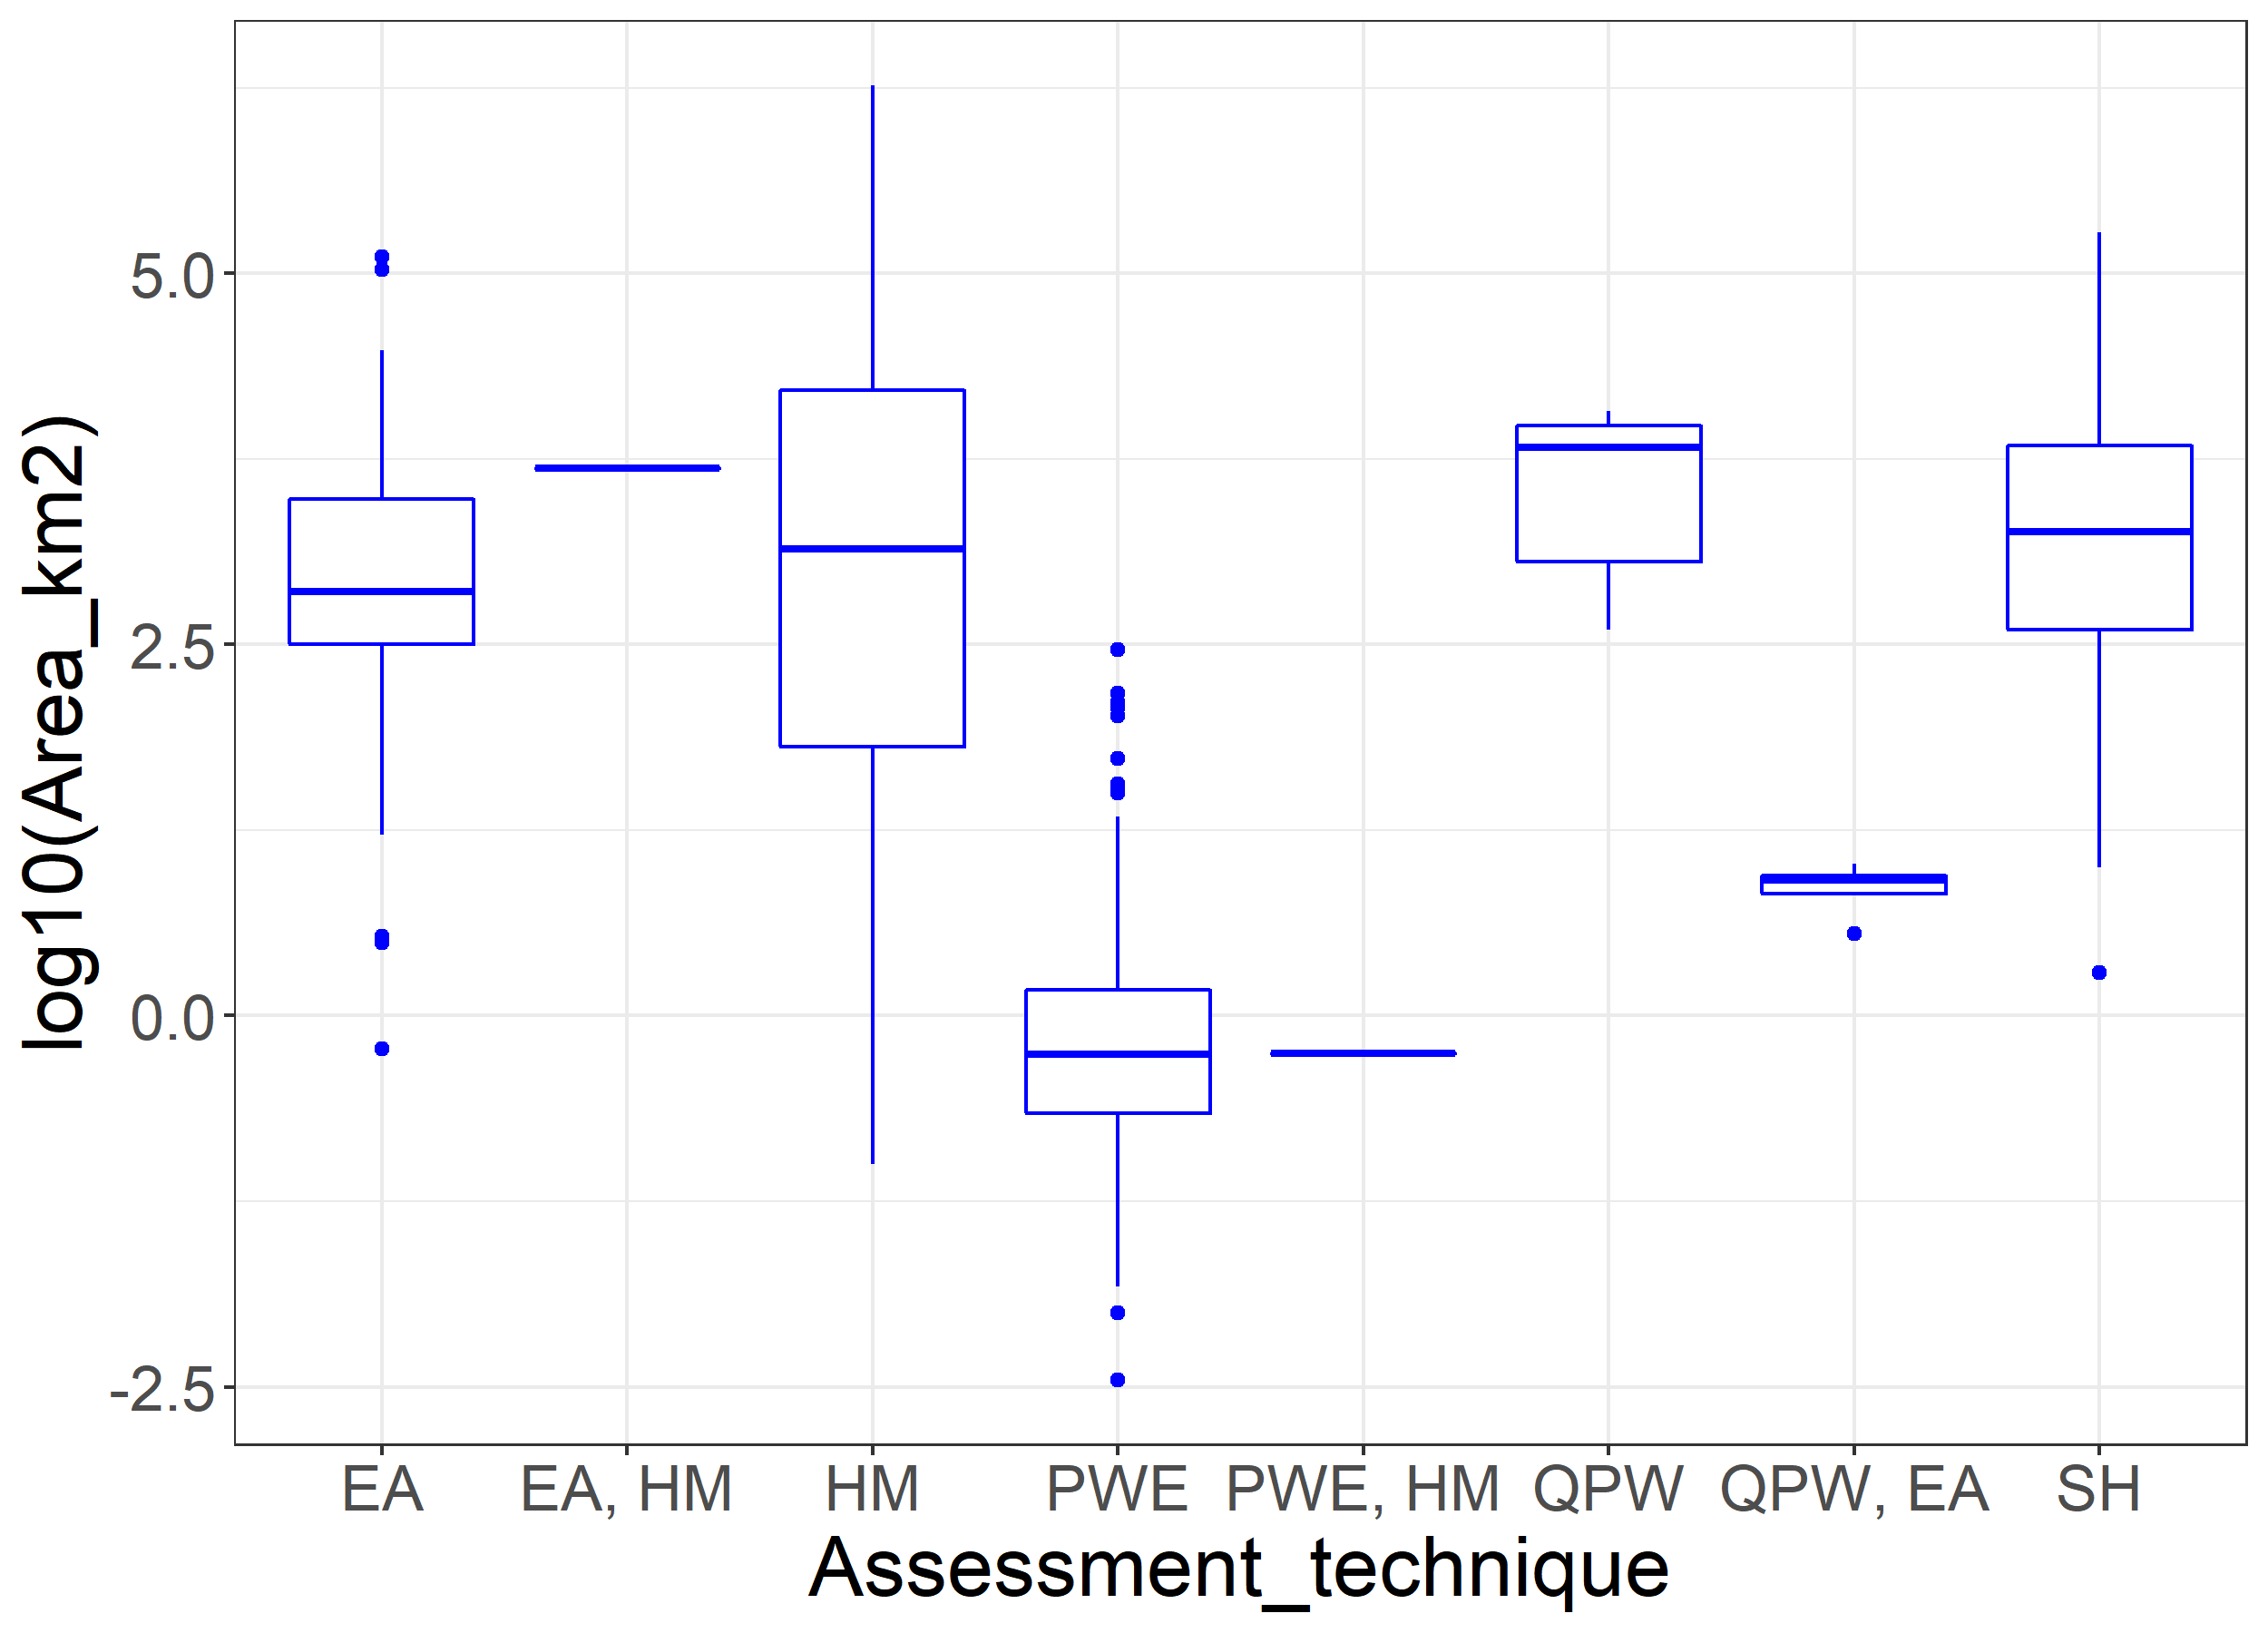
\includegraphics[width=0.9\linewidth]{AssessmentTechnique_byArea} \caption{Boxplot of the log base 10 of the watershed area (in km2) for the different assessment techniques, showing the dominance of small watersheds in the paired watershed experiments}\label{fig:assessment}
\end{figure}

\begin{longtable}[]{@{}
  >{\centering\arraybackslash}p{(\columnwidth - 8\tabcolsep) * \real{0.40}}
  >{\centering\arraybackslash}p{(\columnwidth - 8\tabcolsep) * \real{0.15}}
  >{\centering\arraybackslash}p{(\columnwidth - 8\tabcolsep) * \real{0.17}}
  >{\centering\arraybackslash}p{(\columnwidth - 8\tabcolsep) * \real{0.13}}
  >{\centering\arraybackslash}p{(\columnwidth - 8\tabcolsep) * \real{0.15}}@{}}
\toprule
\begin{minipage}[b]{\linewidth}\centering
~
\end{minipage} & \begin{minipage}[b]{\linewidth}\centering
Estimate
\end{minipage} & \begin{minipage}[b]{\linewidth}\centering
Std. Error
\end{minipage} & \begin{minipage}[b]{\linewidth}\centering
t value
\end{minipage} & \begin{minipage}[b]{\linewidth}\centering
Pr(\textgreater\textbar t\textbar)
\end{minipage} \\
\midrule
\endhead
\textbf{(Intercept)} & -18.71 & 19.02 & -0.98 & 0.33 \\
\textbf{DeltaF\_perc\_pos} & 0.29 & 0.1 & 2.83 & 0 \\
\textbf{Forest\_Signincrease} & -23.26 & 7.15 & -3.25 & 0 \\
\textbf{Precip\_data\_typeOB} & -11.25 & 14.19 & -0.79 & 0.43 \\
\textbf{Precip\_data\_typeSG} & 18.43 & 16.43 & 1.12 & 0.26 \\
\textbf{Assessment\_techniqueHM} & 32.02 & 12.76 & 2.51 & 0.01 \\
\textbf{Assessment\_techniquePWE} & 44.48 & 12.97 & 3.43 & 0 \\
\textbf{Assessment\_techniqueQPW} & 38.12 & 21.21 & 1.8 & 0.07 \\
\textbf{Assessment\_techniqueSH} & 46.79 & 13.17 & 3.55 & 0 \\
\textbf{Forest\_typeCF} & -3.3 & 8.23 & -0.4 & 0.69 \\
\textbf{Forest\_typeMF} & -3.88 & 8.69 & -0.45 & 0.66 \\
\textbf{Hydrological\_regimeSD} & 5.73 & 10.11 & 0.57 & 0.57 \\
\bottomrule
\end{longtable}

\begin{longtable}[]{@{}
  >{\centering\arraybackslash}p{(\columnwidth - 8\tabcolsep) * \real{0.35}}
  >{\centering\arraybackslash}p{(\columnwidth - 8\tabcolsep) * \real{0.10}}
  >{\centering\arraybackslash}p{(\columnwidth - 8\tabcolsep) * \real{0.12}}
  >{\centering\arraybackslash}p{(\columnwidth - 8\tabcolsep) * \real{0.10}}
  >{\centering\arraybackslash}p{(\columnwidth - 8\tabcolsep) * \real{0.14}}@{}}
\toprule
\begin{minipage}[b]{\linewidth}\centering
~
\end{minipage} & \begin{minipage}[b]{\linewidth}\centering
edf
\end{minipage} & \begin{minipage}[b]{\linewidth}\centering
Ref.df
\end{minipage} & \begin{minipage}[b]{\linewidth}\centering
F
\end{minipage} & \begin{minipage}[b]{\linewidth}\centering
p-value
\end{minipage} \\
\midrule
\endhead
\textbf{s(Dryness)} & 3.51 & 9 & 1.96 & 0 \\
\textbf{s(log10(Area\_km2))} & 0.7 & 9 & 0.24 & 0.08 \\
\textbf{s(length)} & 0 & 9 & 0 & 0.99 \\
\bottomrule
\end{longtable}

In drier watersheds, changes in forest cover have greater impact on flow, which is similar to Zhang et al. (2017). This is most likely because in these watersheds the overall flow is surface flow dominated and therefore the buffering that is afforded by the groundwater inputs is not as great. As we don't have a separate variable for groundwater inputs (although this effect is estimated in many studies), we cannot analyse this effect separately.

In contrast to Filoso et al. (2017), we also did not identify an effect of the

Given how skewed Dryness is due to the few watersheds that have very high dryness values, it is worth investigating what excluding these 4 watersheds from the data means for the relationships.

\hypertarget{other-possible-bias-in-the-data}{%
\subsubsection{Other possible bias in the data}\label{other-possible-bias-in-the-data}}

There are further confounding factors in the data, which were also classified by Filoso et al. (2017) and these create biases in the data set that can impact the overall assessment. For example, snow dominated hydrological regimes (SD), which are weakly significant, are dominated by Coniferous Forests (CF), while the majority of the rain dominated regimes are all broadleaf forests (BF). However, the forest type classification is very coarse and does not fully capture possible physiological differences that could affect evapotranspiration and therefore changes in streamflow.

Apart from a difficulty of analysing complex confounding factors in the data, a general limitation of the type of analysis presented is that this work does not consider the spatial arrangement of the forest clearing in the catchments. While for fully or almost fully cleared smaller catchments this might not be an issue, it is perceivable that for larger catchments being partially cleared, a interaction between spatial location and clearing could be a factor in determining the change in streamflow. Clearing head water catchments on shallower soils might have a larger impact than clearing in downstream areas on deeper soils.

\hypertarget{references}{%
\section*{References}\label{references}}
\addcontentsline{toc}{section}{References}

\hypertarget{refs}{}
\begin{CSLReferences}{1}{0}
\leavevmode\vadjust pre{\hypertarget{ref-andreassian2004}{}}%
Andréassian, V., 2004. Waters and forests: From historical controversy to scientific debate. Journal of Hydrology 291, 1--27. doi:\url{https://doi.org/10.1016/j.jhydrol.2003.12.015}

\leavevmode\vadjust pre{\hypertarget{ref-borg1988}{}}%
Borg, H., Bell, R.W., Loh, I.C., 1988. Streamflow and stream salinity in a small water supply catchment in southwest western australia after reforestation. Journal of Hydrology 103, 323--333. doi:\url{https://doi.org/10.1016/0022-1694(88)90141-2}

\leavevmode\vadjust pre{\hypertarget{ref-hewlett1984}{}}%
Bosch, J.M., Hewlett, J.D., 1982. A review of catchment experiments to determine the effect of vegetation changes on water yield and evapotranspiration. Journal of Hydrology 55, 3--23.

\leavevmode\vadjust pre{\hypertarget{ref-brown2013}{}}%
Brown, A.E., Western, A.W., McMahon, T.A., Zhang, L., 2013. Impact of forest cover changes on annual streamflow and flow duration curves. Journal of Hydrology 483, 39--50. doi:\url{http://dx.doi.org/10.1016/j.jhydrol.2012.12.031}

\leavevmode\vadjust pre{\hypertarget{ref-brown2005}{}}%
Brown, A.E., Zhang, L., McMahon, T.A., Western, A.W., Vertessy, R.A., 2005. A review of paired catchment studies for determining changes in water yield resulting from alterations in vegetation. Journal of Hydrology 310, 28--61.

\leavevmode\vadjust pre{\hypertarget{ref-cosandey2005}{}}%
Cosandey, C., Andréassian, V., Martin, C., Didon-Lescot, J.F., Lavabre, J., Folton, N., Mathys, N., Richard, D., 2005. The hydrological impact of the mediterranean forest: A review of french research. Journal of Hydrology 301, 235--249. doi:\url{https://doi.org/10.1016/j.jhydrol.2004.06.040}

\leavevmode\vadjust pre{\hypertarget{ref-filoso2017}{}}%
Filoso, S., Bezerra, M.O., Weiss, K.C.B., Palmer, M.A., 2017. Impacts of forest restoration on water yield: A systematic review. PLOS ONE 12, e0183210. doi:\href{https://doi.org/10.1371/journal.pone.0183210}{10.1371/journal.pone.0183210}

\leavevmode\vadjust pre{\hypertarget{ref-jackson2005}{}}%
Jackson, R.B., Jobbagy, E.G., Avissar, R., Roy, S.B., Barrett, D.J., Cook, C.W., Farley, K.A., Maitre, D.C. le, McCarl, B.A., Murray, B.C., 2005. Trading water for carbon with biological carbon sequestration. Science 310, 1944--1947. doi:\href{https://doi.org/10.1126/science.1119282}{10.1126/science.1119282}

\leavevmode\vadjust pre{\hypertarget{ref-kuczera1987}{}}%
Kuczera, G., 1987. Prediction of water yield reductions following a bushfire in ash-mixed species eucalypt forest. Journal of Hydrology 94, 215--236. doi:\href{https://doi.org/Doi:\%2010.1016/0022-1694(87)90054-0}{Doi: 10.1016/0022-1694(87)90054-0}

\leavevmode\vadjust pre{\hypertarget{ref-pena-arancibia2012}{}}%
Peña-Arancibia, J.L., Dijk, A.I.J.M. van, Guerschman, J.P., Mulligan, M., Bruijnzeel, L.A., McVicar, T.R., 2012. Detecting changes in streamflow after partial woodland clearing in two large catchments in the seasonal tropics. Journal of Hydrology 416-417, 60--71. doi:\url{https://doi.org/10.1016/j.jhydrol.2011.11.036}

\leavevmode\vadjust pre{\hypertarget{ref-roche1981}{}}%
Roche, M., 1981. Watershed investigations for development of forest resources of the amazon region in french guyana. Tropical Agricultural Hydrology. J 75--82.

\leavevmode\vadjust pre{\hypertarget{ref-rodriguez2010}{}}%
Rodriguez, D.A., Tomasella, J., Linhares, C., 2010. Is the forest conversion to pasture affecting the hydrological response of amazonian catchments? Signals in the ji-paraná basin. Hydrological Processes 24, 1254--1269. doi:\url{https://doi.org/10.1002/hyp.7586}

\leavevmode\vadjust pre{\hypertarget{ref-ruprechtetal1991}{}}%
Ruprecht, J.K., Schofield, N.J., Crombie, D.S., Vertessy, R.A., Stoneman, G.L., 1991. Early hydrological response to intense forest thinning in southwestern australia. Journal of Hydrology 127, 261--277. doi:\url{https://doi.org/10.1016/0022-1694(91)90118-2}

\leavevmode\vadjust pre{\hypertarget{ref-thornton2007}{}}%
Thornton, C.M., Cowie, B.A., Freebairn, D.M., Playford, C.L., 2007. The brigalow catchment study: II*. Clearing brigalow (acacia harpophylla) for cropping or pasture increases runoff. Australian Journal of Soil Research 45, 496--511. doi:\href{https://doi.org/doi:10.1071/SR07064}{doi:10.1071/SR07064}

\leavevmode\vadjust pre{\hypertarget{ref-trabucco2018}{}}%
Trabucco, A., Zomer, R.J., 2018. Global aridity index and potential evapo-transpiration (ET0) climate database v2. CGIAR consortium for spatial information(CGIAR-CSI).

\leavevmode\vadjust pre{\hypertarget{ref-wood2006}{}}%
Wood, S., 2006. Generalized additive models: An introduction with r. CRC Press, Boca Raton, FL.

\leavevmode\vadjust pre{\hypertarget{ref-zhang2011}{}}%
Zhang, L., Zhao, F., Chen, Y., Dixon, R.N.M., 2011. Estimating effects of plantation expansion and climate variability on streamflow for catchments in australia. Water Resources Research 47, W12539. doi:\href{https://doi.org/10.1029/2011wr010711}{10.1029/2011wr010711}

\leavevmode\vadjust pre{\hypertarget{ref-zhang2017}{}}%
Zhang, M., Liu, N., Harper, R., Li, Q., Liu, K., Wei, X., Ning, D., Hou, Y., Liu, S., 2017. A global review on hydrological responses to forest change across multiple spatial scales: Importance of scale, climate, forest type and hydrological regime. Journal of Hydrology 546, 44--59. doi:\url{https://doi.org/10.1016/j.jhydrol.2016.12.040}

\leavevmode\vadjust pre{\hypertarget{ref-zhao2010}{}}%
Zhao, F., Zhang, L., Xu, Z., Scott, D.F., 2010. Evaluation of methods for estimating the effects of vegetation change and climate variability on streamflow. Water Resources Research 46, W03505. doi:\href{https://doi.org/10.1029/2009wr007702}{10.1029/2009wr007702}

\leavevmode\vadjust pre{\hypertarget{ref-zhou2015}{}}%
Zhou, G., Wei, X., Chen, X., Zhou, P., Liu, X., Xiao, Y., Sun, G., Scott, D.F., Zhou, S., Han, L., Su, Y., 2015. Global pattern for the effect of climate and land cover on water yield. Nature Communications 6, 5918. doi:\href{https://doi.org/10.1038/ncomms6918}{10.1038/ncomms6918}

\leavevmode\vadjust pre{\hypertarget{ref-zhou2010}{}}%
Zhou, G., Wei, X., Luo, Y., Zhang, M., Li, Y., Qiao, Y., Liu, H., Wang, C., 2010. Forest recovery and river discharge at the regional scale of guangdong province, china. Water Resources Research 46. doi:\url{https://doi.org/10.1029/2009WR008829}

\end{CSLReferences}


\end{document}
